% !Mode:: "TeX:UTF-8"
\def\usewhat{pdflatex}                               % 定义编译方式 dvipdfmx 或者 pdflatex,默认为 dvipdfmx
                                                     % 方式编译,如果需要修改,只需改变花括号中的内容即可。
\documentclass[12pt,openany,a4paper,twoside]{book} %原本的设置
%\documentclass[12pt,openany,twoside]{book}           % 本科生毕业论文通常采用单页排版
% !Mode:: "TeX:UTF-8"
%  Authors: 张井   Jing Zhang: prayever@gmail.com     天津大学2010级管理与经济学部信息管理与信息系统专业硕士生
%           余蓝涛 Lantao Yu: lantaoyu1991@gmail.com  天津大学2008级精密仪器与光电子工程学院测控技术与仪器专业本科生

%%%%%%%%%% Package %%%%%%%%%%%%
\usepackage{graphicx}                       % 支持插图处理
\usepackage[a4paper,text={146.4true mm,239.2 true mm},top= 26.2true mm,left=31.8 true mm,head=6true mm,headsep=6.5true mm,foot=16.5true mm]{geometry}
                                            % 支持版面尺寸设置
\usepackage[squaren]{SIunits}               % 支持国际标准单位

\usepackage{titlesec}                       % 控制标题的宏包
\usepackage{titletoc}                       % 控制目录的宏包
\usepackage{fancyhdr}                       % fancyhdr宏包 支持页眉和页脚的相关定义
\usepackage[UTF8]{ctex}                     % 支持中文显示
\usepackage{CJKpunct}                       % 精细调整中文的标点符号
\usepackage{color}                          % 支持彩色
\usepackage{amsmath}                        % AMSLaTeX宏包 用来排出更加漂亮的公式
\usepackage{amssymb}                        % 数学符号生成命令
\usepackage[below]{placeins}    %允许上一个section的浮动图形出现在下一个section的开始部分,还提供\FloatBarrier命令,使所有未处理的浮动图形立即被处理
\usepackage{multirow}                       % 使用Multirow宏包,使得表格可以合并多个row格
\usepackage{booktabs}                       % 表格,横的粗线;\specialrule{1pt}{0pt}{0pt}
\usepackage{longtable}                      % 支持跨页的表格。
\usepackage{tabularx}                       % 自动设置表格的列宽
\usepackage{subfigure}                      % 支持子图 %centerlast 设置最后一行是否居中
\usepackage[subfigure]{ccaption}            % 支持子图的中文标题
\usepackage[sort&compress,numbers]{natbib}  % 支持引用缩写的宏包
\usepackage{enumitem}                       % 使用enumitem宏包,改变列表项的格式
\usepackage{calc}                           % 长度可以用+ - * / 进行计算
\usepackage{txfonts}                        % 字体宏包
\usepackage{bm}                             % 处理数学公式中的黑斜体的宏包
\usepackage[amsmath,thmmarks,hyperref]{ntheorem}  % 定理类环境宏包,其中 amsmath 选项用来兼容 AMS LaTeX 的宏包
\usepackage{CJKnumb}                        % 提供将阿拉伯数字转换成中文数字的命令
\usepackage{indentfirst}                    % 首行缩进宏包
\usepackage{CJKutf8}                        % 用在UTF8编码环境下,它可以自动调用CJK,同时针对UTF8编码作了设置
%\usepackage{hypbmsec}                      % 用来控制书签中标题显示内容
%\usepackage{enumerate}                      % 用于控制排序列表的编号样式
\newcommand{\tabincell}[2]{\begin{tabular}{@{}#1@{}}#2\end{tabular}}
\usepackage{xcolor}
%支持代码环境
\usepackage{listings}
\lstset{numbers=left,
language=[ANSI]{C},
numberstyle=\tiny,
extendedchars=false,
showstringspaces=false,
breakatwhitespace=false,
breaklines=true,
captionpos=b,
keywordstyle=\color{blue!70},
commentstyle=\color{red!50!green!50!blue!50},
frame=shadowbox,
rulesepcolor=\color{red!20!green!20!blue!20}
}
%支持算法环境
\usepackage[longend,linesnumbered,boxed,ruled,lined]{algorithm2e}
%\usepackage{algorithmic}

\usepackage{array}
\newcommand{\PreserveBackslash}[1]{\let\temp=\\#1\let\\=\temp}
\newcolumntype{C}[1]{>{\PreserveBackslash\centering}p{#1}}
\newcolumntype{R}[1]{>{\PreserveBackslash\raggedleft}p{#1}}
\newcolumntype{L}[1]{>{\PreserveBackslash\raggedright}p{#1}}

% 生成有书签的 pdf 及其生成方式。通常可以在 tjumain.tex 文件的第一行选择 pdflatex 或者是 dvipdfmx 编译手段。如果选择前者,则使用 pdflatex + pdflatex 编译; 如果选择后者,在编译的时候选择 latex + bibtex + latex + latex 编译。出现混淆的时候,系统会报错。
% 如果您的pdf制作中文书签有乱码使用如下命令,就可以解决了
\def\atemp{dvipdfmx}\ifx\atemp\usewhat
\usepackage[dvipdfmx,unicode,               % dvipdfmx 编译, 加入了中文复制,粘贴支持引擎。
            pdfstartview=FitH,
            bookmarksnumbered=true,
            bookmarksopen=true,
            colorlinks=false,
            pdfborder={0 0 1},
            citecolor=blue,
            linkcolor=black,
            anchorcolor=green,
            urlcolor=blue,
            breaklinks=true
            ]{hyperref}
\fi

\def\atemp{pdflatex}\ifx\atemp\usewhat
\usepackage{cmap}                           % pdflatex 编译时,可以生成可复制、粘贴的中文 PDF 文档, 缺点是在Windows上显示时效果不大好,字体发虚
\usepackage[pdftex,unicode,
            %CJKbookmarks=true,
            bookmarksnumbered=true,
            bookmarksopen=true,
            colorlinks=false,
            pdfborder={0 0 0},%pdfborder={0 0 1}就能显示红色框
            citecolor=blue,
            linkcolor=red,
            anchorcolor=green,
            urlcolor=blue,
            breaklinks=true
            ]{hyperref}
\fi

\usepackage{setspace}   % 用于目录设置行距


\usepackage{caption}

                                % 定义本文所使用宏包
\usepackage{graphicx}
\usepackage{subfigure}
\usepackage{epstopdf}                                 %支持eps图片转换成PDF格式
\usepackage{tipa}
\usepackage{multirow}
\graphicspath{{figures/}}                            % 定义所有的 .eps 文件在 figures 子目录下
\begin{document}                                     % 开始全文
\begin{CJK*}{UTF8}{song}                             % 开始中文字体使用
% !Mode:: "TeX:UTF-8"

%%%%%%%%%%%%%%%%% Fonts Definition and Basics %%%%%%%%%%%%%%%%%
\newcommand{\song}{\CJKfamily{song}}    % 宋体
\newcommand{\fs}{\CJKfamily{fs}}        % 仿宋体
\newcommand{\kai}{\CJKfamily{kai}}      % 楷体
\newcommand{\hei}{\CJKfamily{hei}}      % 黑体
\newcommand{\li}{\CJKfamily{li}}        % 隶书
\newcommand{\chuhao}{\fontsize{28pt}{28pt}\selectfont}       % 初号, 单倍行距
\newcommand{\yihao}{\fontsize{26pt}{26pt}\selectfont}       % 一号, 单倍行距
\newcommand{\xiaoyi}{\fontsize{24pt}{24pt}\selectfont}      % 小一, 单倍行距
\newcommand{\erhao}{\fontsize{22pt}{1.25\baselineskip}\selectfont}       % 二号, 1.25倍行距
\newcommand{\xiaoer}{\fontsize{18pt}{18pt}\selectfont}      % 小二, 单倍行距
\newcommand{\sanhao}{\fontsize{16pt}{16pt}\selectfont}      % 三号, 单倍行距
\newcommand{\xiaosan}{\fontsize{15pt}{15pt}\selectfont}     % 小三, 单倍行距
\newcommand{\sihao}{\fontsize{14pt}{14pt}\selectfont}       % 四号, 单倍行距
\newcommand{\xiaosi}{\fontsize{12pt}{12pt}\selectfont}      % 小四, 单倍行距
\newcommand{\wuhao}{\fontsize{10.5pt}{10.5pt}\selectfont}   % 五号, 单倍行距
\newcommand{\xiaowu}{\fontsize{9pt}{9pt}\selectfont}        % 小五, 单倍行距

\CJKtilde  % 重新定义了波浪符~的意义
\newcommand\prechaptername{第}
\newcommand\postchaptername{章}

\punctstyle{hangmobanjiao}             % 调整中文字符的表示,行内占一个字符宽度,行尾占半个字符宽度

% 调整罗列环境的布局
\setitemize{leftmargin=3em,itemsep=0em,partopsep=0em,parsep=0em,topsep=-0em}
\setenumerate{leftmargin=3em,itemsep=0em,partopsep=0em,parsep=0em,topsep=0em}

% 避免宏包 hyperref 和 arydshln 不兼容带来的目录链接失效的问题。
\def\temp{\relax}
\let\temp\addcontentsline
\gdef\addcontentsline{\phantomsection\temp}

% 自定义项目列表标签及格式 \begin{publist} 列表项 \end{publist}
\renewcommand{\labelenumi}{(\arabic{enumi})}               %定义列表项目符号为(1)格式
\newcounter{pubctr} %自定义新计数器
\newenvironment{publist}{%%%%%定义新环境
\begin{list}{[\arabic{pubctr}]} %%标签格式
    {
     \usecounter{pubctr}
     \setlength{\leftmargin}{2.5em}   % 左边界 \leftmargin =\itemindent + \labelwidth + \labelsep
     \setlength{\itemindent}{0em}     % 标号缩进量
     \setlength{\labelsep}{1em}       % 标号和列表项之间的距离,默认0.5em
     \setlength{\rightmargin}{0em}    % 右边界
     \setlength{\topsep}{0ex}         % 列表到上下文的垂直距离
     \setlength{\parsep}{0ex}         % 段落间距
     \setlength{\itemsep}{0ex}        % 标签间距
     \setlength{\listparindent}{0pt}  % 段落缩进量
    }}
{\end{list}}

\makeatletter
\renewcommand\normalsize{
  \@setfontsize\normalsize{12pt}{12pt} % 小四对应 12 pt
  \setlength\abovedisplayskip{4pt}
  \setlength\abovedisplayshortskip{4pt}
  \setlength\belowdisplayskip{\abovedisplayskip}
  \setlength\belowdisplayshortskip{\abovedisplayshortskip}
  \let\@listi\@listI}
%\def\defaultfont{\renewcommand{\baselinestretch}{2.0}\normalsize\selectfont} % 设置行距
\def\defaultfont{\renewcommand{\baselinestretch}{2.0}\normalsize}
\renewcommand{\CJKglue}{\hskip -0.1 pt plus 0.08\baselineskip} % 控制字间距,使每行 34 个汉字
\makeatother
\setlength{\parskip}{3pt plus.1pt minus.1pt}  % 段落之间的竖直距离


%%%%%%%%%%%%% Contents %%%%%%%%%%%%%%%%%
\renewcommand{\contentsname}{目\qquad 录}
\setcounter{tocdepth}{1} % 控制目录深度   //只显示两级目录
\titlecontents{chapter}[2em]{\vspace{.5\baselineskip}\sihao\song}
             %{\prechaptername\CJKnumber{\thecontentslabel}\postchaptername\qquad}{}   %让目录章节使用“第一章”
             {\prechaptername~\thecontentslabel~\postchaptername\quad}{}               %让目录章节使用“第1章”
             {\hspace{.5em}\titlerule*[5pt]{$\cdot$}\xiaosi\contentspage}
\titlecontents{section}[3em]{\vspace{.25\baselineskip}\xiaosi\song}
             {\thecontentslabel\quad}{}
             {\hspace{.5em}\titlerule*[5pt]{$\cdot$}\xiaosi\contentspage}
\titlecontents{subsection}[4em]{\vspace{.25\baselineskip}\xiaosi\song}
             {\thecontentslabel\quad}{}
             {\hspace{.5em}\titlerule*[5pt]{$\cdot$}\xiaosi\contentspage}

%%%%%%%%%% Chapter and Section %%%%%%%%%%%%%
\setcounter{secnumdepth}{4}
\setlength{\parindent}{2em}
\renewcommand{\chaptername}{\prechaptername\CJKnumber{\thechapter}\postchaptername}     %章名使用“第一章”
\renewcommand{\chaptername}{\prechaptername~\thechapter~\postchaptername}               %章名使用“第1章”
%\titleformat{\chapter}{\centering\xiaoer\bfseries}{\hei\chaptername}{2em}{}
\titleformat{\chapter}{\centering\erhao\hei}{\chaptername}{2em}{}
\titlespacing{\chapter}{0pt}{0.1\baselineskip}{0.8\baselineskip}
\titleformat{\section}{\xiaosan\hei}{\thesection}{1em}{}
\titlespacing{\section}{0pt}{0.15\baselineskip}{0.25\baselineskip}
\titleformat{\subsection}{\sihao\hei}{\thesubsection}{1em}{}
\titlespacing{\subsection}{0pt}{0.1\baselineskip}{0.3\baselineskip}
\titleformat{\subsubsection}{\sihao\hei}{\thesubsubsection}{1em}{}
\titlespacing{\subsubsection}{0pt}{0.05\baselineskip}{0.1\baselineskip}


%%%%%%%%%% Table, Figure and Equation %%%%%%%%%%%%%%%%%
\renewcommand{\tablename}{表}                                     % 插表题头
\renewcommand{\figurename}{图}                                    % 插图题头
\renewcommand{\thefigure}{\arabic{chapter}-\arabic{figure}}       % 使图编号为 7-1 的格式 %\protect{~}
%\renewcommand{\thesubfigure}{\alph{subfigure})}                  % 使子图编号为 a) 的格式
\renewcommand{\thesubfigure}{(\alph{subfigure})}                  % 使子图编号为 (a) 的格式
\renewcommand{\thesubtable}{(\alph{subtable})}                    % 使子表编号为 (a) 的格式
\renewcommand{\thetable}{\arabic{chapter}-\arabic{table}}         % 使表编号为 7-1 的格式
\renewcommand{\theequation}{\arabic{chapter}-\arabic{equation}}   % 使公式编号为 7-1 的格式

\makeatletter
	% 使子图引用也是7-1a)或7-1(a)的形式
	\renewcommand{\p@subfigure}{\thefigure}
\makeatother

%%%%%% 定制浮动图形和表格标题样式 %%%%%%
\makeatletter
\long\def\@makecaption#1#2{
   \vskip\abovecaptionskip
   \sbox\@tempboxa{\centering\wuhao\song{#1\quad #2} }
   \ifdim \wd\@tempboxa >\hsize
     \centering\wuhao\song{#1\qquad #2} \par
   \else
     \global \@minipagefalse
     \hb@xt@\hsize{\hfil\box\@tempboxa\hfil}
   \fi
   \vskip\belowcaptionskip}
\makeatother
\captiondelim{~~~~} %用来控制longtable表头分隔符

\setlength{\floatsep}{10pt plus 3pt minus 2pt}      % 图形之间或图形与正文之间的距离
\setlength{\abovecaptionskip}{5pt plus.1pt minus.1pt} % 图形中的图与标题之间的距离
\setlength{\belowcaptionskip}{3pt plus.1pt minus.1pt} % 表格中的表与标题之间的距离


%%%%%%%%%% Theorem Environment %%%%%%%%%%%%%%%%%
\theoremstyle{plain}
\theorembodyfont{\song}%\rmfamily}
\theoremheaderfont{\hei\bfseries}
\newtheorem{theorem}{定理~}[chapter]
\newtheorem{lemma}{引理~}[chapter]
\newtheorem{axiom}{公理~}[chapter]
\newtheorem{proposition}{命题~}[chapter]
\newtheorem{prop}{性质~}[chapter]
\newtheorem{corollary}{推论~}[chapter]
\newtheorem{conclusion}{结论~}[chapter]
\newtheorem{definition}{定义~}[chapter]
\newtheorem{conjecture}{猜想~}[chapter]
\newtheorem{example}{例~}[chapter]
\newtheorem{remark}{注~}[chapter]
%\newtheorem{algorithm}{算法~}[chapter]
\newenvironment{proof}{\noindent{\hei 证明:}}{\hfill $ \square $ \vskip 4mm}
\theoremsymbol{$\square$}

\renewcommand{\algorithmcfname}{算法}


%%%%%%%%%% Page: number, header and footer  %%%%%%%%%%%%%%%%%

%\frontmatter 或 \pagenumbering{roman}
%\mainmatter 或 \pagenumbering{arabic}
\makeatletter
\renewcommand\frontmatter{\clearpage
  \@mainmatterfalse
  }
\makeatother

%%%%%%%%%%%% References %%%%%%%%%%%%%%%%%
\renewcommand{\bibname}{参考文献}
% 重定义参考文献样式,来自thu
\makeatletter
\renewenvironment{thebibliography}[1]{
    \titleformat{\chapter}{\raggedright\sihao\hei}{\chaptername}{2em}{}
   \chapter*{\bibname}
   \wuhao
   \list{\@biblabel{\@arabic\c@enumiv}}
        {\renewcommand{\makelabel}[1]{##1\hfill}
         \settowidth\labelwidth{0 cm}
         \setlength{\labelsep}{0pt}
         \setlength{\itemindent}{0pt}
         \setlength{\leftmargin}{\labelwidth+\labelsep}
         \addtolength{\itemsep}{-0.7em}
         \usecounter{enumiv}
         \let\p@enumiv\@empty
         \renewcommand\theenumiv{\@arabic\c@enumiv}}
    \sloppy\frenchspacing
    \clubpenalty4000
    \@clubpenalty \clubpenalty
    \widowpenalty4000
    \interlinepenalty4000
    \sfcode`\.\@m}
   {\def\@noitemerr
     {\@latex@warning{Empty `thebibliography' environment}}
    \endlist\frenchspacing}
\makeatother

\addtolength{\bibsep}{-0.5em}     % 缩小参考文献间的垂直间距
\setlength{\bibhang}{2em}         % 每个条目自第二行起缩进的距离



% 参考文献引用作为上标出现
%\newcommand{\citeup}[1]{\textsuperscript{\cite{#1}}}
\makeatletter
    \def\@cite#1#2{\textsuperscript{[{#1\if@tempswa , #2\fi}]}}
\makeatother
%% 引用格式
\bibpunct{[}{]}{,}{s}{}{,}

%%%%%%%%%%%% Cover %%%%%%%%%%%%%%%%%
% 封面、摘要、版权、致谢格式定义
\makeatletter
\def\ctitle#1{\def\@ctitle{#1}}\def\@ctitle{}
\def\etitle#1{\def\@etitle{#1}}\def\@etitle{}
\def\csubject#1{\def\@csubject{#1}}\def\@csubject{}
\def\esubject#1{\def\@esubject{#1}}\def\@esubject{}
\def\cauthor#1{\def\@cauthor{#1}}\def\@cauthor{}
\def\eauthor#1{\def\@eauthor{#1}}\def\@eauthor{}
\def\csupervisor#1{\def\@csupervisor{#1}}\def\@csupervisor{}
\def\esupervisor#1{\def\@esupervisor{#1}}\def\@esupervisor{}
\def\cdate#1{\def\@cdate{#1}}\def\@cdate{}
\long\def\cabstract#1{\long\def\@cabstract{#1}}\long\def\@cabstract{}
\long\def\eabstract#1{\long\def\@eabstract{#1}}\long\def\@eabstract{}
\def\ckeywords#1{\def\@ckeywords{#1}}\def\@ckeywords{}
\def\ekeywords#1{\def\@ekeywords{#1}}\def\@ekeywords{}
\def\cheading#1{\def\@cheading{#1}}\def\@cheading{}


\pagestyle{fancy}
  \fancyhf{}
  \renewcommand{\chaptermark}[1]%
    {\markboth{\chaptername \ #1}{}}            % \chaptermark 去掉章节标题中的数字
  %\fancyhead[C]{\song\wuhao \@cheading}  % 页眉
  %\fancyhead[RO]{\song\xiaosi \leftmark}
  %\fancyhead[LE]{\song\xiaosi \@ctitle}
  \lhead{\song\wuhao \@ctitle}  % 左页眉
  \rhead{\song\wuhao \leftmark}    % 右页眉
  \fancyfoot[C]{\song\wuhao ~\thepage~}
\newlength{\@title@width}

% 定义封面
\def\makecover{
%\cleardoublepage%
   \phantomsection
    \pdfbookmark[-1]{\@ctitle}{ctitle}

\begin{titlepage}
\vspace*{10pt}
\begin{center}

  \vspace*{10pt}
  \hei\chuhao{\textbf{中山大学硕士学位论文}}

  \vspace*{60pt}
  \song\xiaoer\textbf{\@ctitle}

  \xiaoer{\textbf{\@etitle}}

  \begin{spacing}{2.0}
  \vspace*{42pt}
  \setlength{\@title@width}{6cm}
  {\sihao\kai{{

  \begin{tabular}{lc}
    学~~位~~申~~请~~人:   &  \underline{\makebox[\@title@width][c]{\@cauthor}} \\
    导师姓名及职称:       &  \underline{\makebox[\@title@width][c]{\@csupervisor}} \\
    专~~~~业~~~~名~~~~称: &  \underline{\makebox[\@title@width][c]{\@csubject}}\\
  \end{tabular}}}
 }

 \end{spacing}

  \vspace*{10pt}


 \begin{spacing}{2.0}
 \vspace*{10pt}
  \setlength{\@title@width}{5cm}
  {\sanhao\kai{{
  \begin{tabular}{lc}
    答辩委员会主席(签名):  &  \underline{\makebox[\@title@width][c]{~}} \\
    答辩委员会委员(签名):  &  \underline{\makebox[\@title@width][c]{~}} \\
    ~ &  \underline{\makebox[\@title@width][c]{~}}\\
    ~ &  \underline{\makebox[\@title@width][c]{~}}\\
    ~ &  \underline{\makebox[\@title@width][c]{~}}\\
    ~ &  \underline{\makebox[\@title@width][c]{~}}\\
  \end{tabular}}}
 }
 \end{spacing}
 \vspace*{20pt}

  \vspace*{21pt}

\kai\sihao{\@cdate}
\end{center}
\end{titlepage}

 %空白页
\newpage
\thispagestyle{empty}
\mbox{}

%%%%%%%%%%%%%%%%   Originality Statement  %%%%%%%%%%%%%%%%%%%%%%%
\clearpage
\pdfbookmark[0]{论文原创性声明}{originality}
\chapter*{\centering\sanhao\song\bfseries 论文原创性声明}
\song\defaultfont
本人郑重声明:所呈交的学位论文,是本人在导师的指导下,独立进行研究工作所取得的成果。除文中已经注明引用的内容外,本论文不包含任何其他个人或集体已经发表或撰写过的作品成果。对本文的研究作出重要贡献的个人和集体,均已在文中以明确方式标明。本人完全意识到本声明的法律结果由本人承担。

\vspace*{40pt}
\begin{flushright}
\setlength{\@title@width}{5cm}
  {\sihao\song{
  \begin{tabular}{lc}
    学位论文作者签名:           &  \underline{\makebox[\@title@width][c]{~}} \\
    \qquad\qquad\qquad 日~~期:  &  \underline{\makebox[\@title@width][c]{~}} \\
  \end{tabular}}
 }
\end{flushright}

%%%%%%%%%%%%%%%%   Authorization Statement  %%%%%%%%%%%%%%%%%%%%%%%
\vspace*{60pt}
\pdfbookmark[0]{学位论文使用授权声明}{authorization}
\begin{center}
  \sanhao\song\bfseries{学位论文使用授权声明}
\end{center}

\song\defaultfont
本人完全了解中山大学有关保留、使用学位论文的规定,即:学校有权保留学位论文并向国家主管部门或其指定机构送交论文的电子版和纸质版,有权将学位论文用于非赢利目的的少量复制并允许论文进入学校图书馆、院系资料室被查阅,有权将学位论文的内容编入有关数据库进行检索,可以采用复印、缩印或其他方法保存学位论文。

\vspace*{40pt}
\begin{center}
\setlength{\@title@width}{5cm}
  {\sihao\song{
  \begin{tabular}{ll}
    学位论文作者签名: \qquad\qquad\qquad\qquad\qquad  &  导师签名: \qquad\qquad\qquad\\
    日期: \qquad 年\qquad 月\qquad 日     &  日期: \qquad 年\qquad 月\qquad 日 \\
  \end{tabular}}
 }
\end{center}
\thispagestyle{empty}   % 去掉页码

 %空白页
\newpage
\thispagestyle{empty}
\mbox{}


%%%%%%%%%%%%%%%%%%%   Abstract and Keywords  %%%%%%%%%%%%%%%%%%%%%%%
\clearpage
\setcounter{page}{1} % 重新开始页码
\pagenumbering{Roman} %罗马数字页码
\markboth{摘~要}{摘~要}
\pdfbookmark[0]{摘~~要}{cabstract}
\newpage

\begin{flushleft}
\setlength{\@title@width}{5cm}
  {\wuhao\song{
  \begin{tabular}{ll}
    论文题目:  & \@ctitle  \\ %&  %\@ctitle\\
    专~~~~~~业:  &  \@csubject \\
    硕~~士~~生:  &  \@cauthor \\
    指导老师:    &  \@csupervisor \\
  \end{tabular}}
 }
\end{flushleft}

%\addcontentsline{toc}{chapter}{摘~要}
\vspace{\baselineskip}
\begin{center}
\xiaoer\hei\bfseries 摘\qquad 要
\end{center}

\song\defaultfont
\@cabstract
\vspace{\baselineskip}

\hangafter=1\hangindent=52.3pt\noindent
{\hei\xiaosi 关键词:} \@ckeywords
%\thispagestyle{plain}

% 空白页
\clearpage{\pagestyle{empty}\cleardoublepage}
%\newpage
%\thispagestyle{empty}
%\mbox{}

%%%%%%%%%%%%%%%%%%%   English Abstract  %%%%%%%%%%%%%%%%%%%%%%%%%%%%%%
\clearpage
%\fancypagestyle{plain}{                             %设置英文摘要页眉的论文题目为英文
%\fancyhead{}
%\fancyhead[RO]{\wuhao \@etitle}  % 左页眉
%\fancyhead[LE]{\wuhao \leftmark}    % 右页眉
%\fancyfoot[C]{\song\xiaowu~\thepage~}
%}
%\thispagestyle{plain}
%\phantomsection
\markboth{ABSTRACT}{ABSTRACT}
\pdfbookmark[0]{ABSTRACT}{eabstract}
%\addcontentsline{toc}{chapter}{ABSTRACT}   % 摘要不加到目录中
\newpage

\begin{flushleft}           % 如果英文title太长,手动分成两行
\setlength{\@title@width}{5cm}
  {\wuhao{
  \begin{tabular}{lp{0.8\textwidth}}
    Title:  & \@etitle \\
    Major:      &  \@esubject \\
    Name:       &  \@eauthor \\
    Supervisor: &  \@esupervisor \\
  \end{tabular}}
 }
\end{flushleft}

\vspace{\baselineskip}
\begin{center}
\sanhao{\bf{Abstract}}
\end{center}

%\vspace{\baselineskip}
\@eabstract
\vspace{\baselineskip}

\hangafter=1\hangindent=52.3pt\noindent
{\textbf{Keywords:}} \@ekeywords
%\thispagestyle{plain}

% 空白页
\clearpage{\pagestyle{empty}\cleardoublepage}
}
\makeatother
                                 % 完成对论文各个部分格式的设置

\frontmatter                                         % 以下是论文导言部分,包括论文的封面,中英文摘要和中文目录
%\fancypagestyle{plain}{
%\fancyhf{}
%\lhead{\song\wuhao \@ctitle}  % 左页眉
%\rhead{\song\wuhao \leftmark}    % 右页眉
%\fancyfoot[C]{\song\xiaowu~\thepage~}
%\renewcommand{\headrulewidth}{0 pt}
%}

%%%%%%%%%%   封面   %%%%%%%%%%
% !Mode:: "TeX:UTF-8"

%%  可通过增加或减少 setup/format.tex中的
%%  第274行 \setlength{\@title@width}{8cm}中 8cm 这个参数来 控制封面中下划线的长度。
\cheading{中山大学硕士学位论文}      % 设置正文的页眉,需要填上对应的毕业年份
\ctitle{基于消息传递机制的社会关系理解方法研究}    % 封面用论文标题,自己可手动断行
\etitle{Social Relationship Understanding via Message Passing Mechanism}    %论文英文标题
\csubject{工程(软件工程)}   % 专业名称
\esubject{Engineering (software engineering) }
\cauthor{
李雷来
}            % 学生姓名
\eauthor{
Leilai Li
}
\csupervisor{
xxx
}        % 导师姓名
\esupervisor{
xxx
}

%\cdate{\the\year~\the\month~月~\the\day~日}
\cdate{二零一九~年~五~月~九~日}

\cabstract{
本文致力于研究社会关系理解问题,社会关系理解是为了推断出一个给定场景中人之间的社会关系。近来关系理解在计算机视觉领域受到极大的关注,任务的效果也随着深度学习方法的发展得到了快速的提高,但是现有的工作主要通过挖掘人对的图像基本特征,或者引入物体和关系共现频率的先验知识来提升效果。这些工作将图片中的每个人对的关系检测独立的看待,并没有考虑到这些人对之间的相互关系。因此,在社会关系理解任务中很自然的考虑到这样的交互信息。例如,如果一张图片两个人对是朋友,那么第三个人对的关系往往是朋友或至少是其他亲密的社会关系,而不是无关系。为了捕捉到这样交互的线索,本文提出社会关系图谱的概念,以及一个端到端的可训练的人对关系网络,采用RNNs来实现人对之间的消息传递达到推理的目的,提高关系的分类结果。

在PPRN中,本文提出一个消息传递和消息池化模块来实现不同人对之间的信息传递,达到不同人对关系互相约束的目的,以及实现了一个基于注意力机制来结合周边物体特征的模块。在这个过程中,消息传递和池化这两个模块不断迭代,再融合区域生成网络生成的物体区域的图像特征,最后进行分类优化。

在实验中,本文在两个大规模数据集中验证了PPRN模型的有效性,这两个公开数据集包括三个不同的关系粒度,接着进行了具体案例的分析。实现结果表明了PPRN模型在与其他基准模型的对比中取得了最优的结果,同时说明了在视觉关系理解任务中考虑不同人对间相互影响的重要性。
}
\ckeywords{社会关系理解,消息传递,注意力机制,神经网络}

\eabstract{
This paper focuses on social relationships understanding which aims at inferring the social relations among people in a given scene. Relationship Understanding has attracted increasing attention in computer vision recently. Great progress has been made since the rise of deep learning. However, previous works mainly improves the results by mining the basic features of person pair or introducing prior knowledge of object and relationship co-occurrence frequencies, without taking into account the interaction of different pairs. It is natural to consider these interaction cues, {\it i.e.,} the mutual influence of multiple person pairs, in social relationship understanding. For instance, if two person pairs in an image are ``Friends'', then the third pair is always ``Friends'' or at least other similar relations but not ``No Relation''. Therefore, to capture these interaction cues, we propose the concept of social relationship graph, and a novel end-to-end trainable Person-Pair Relation Network ({\it PPRN}) using standard RNNs, a inference network that learns iteratively to improve its predictions via message passing among person pair nodes.

In PPRN model, we provide a message passing and message pooling module to implements the message passing between various person pairs,achieving the purpose of the mutual restraint between different person pair, and we also implements a attention module to combine the contextual object feature. In this process, the first step is to iterate the two modules of message passing and pooling between person pair's relationships, and then combine the image features of object bounding box generated by the region proposal network, and finally optimization.

In the experiments, we evaluate our model in two large-scale datasets, and the two datasets contain three relational granularity, and further analyze by case studies. Experimental results demonstrate that our model outperforms baselines, which justifies the significance of considering the interaction between various person pairs in social relationship understanding.
}

\ekeywords{social relationship understanding,message passing,attention mechanism,neural network}

\makecover

\clearpage



                                % 封面

%%%%%%%%%%   目录   %%%%%%%%%%
\defaultfont
\clearpage{\pagestyle{empty}\cleardoublepage}       %本有
%\setcounter{page}{1}                                % 单独从 1 开始编页码
%\pagenumbering{Roman}
\titleformat{\chapter}{\centering\sanhao\hei}{\chaptername}{2em}{} % 设置目录两字的格式
\pdfbookmark[0]{目~~录}{mulu}
\fancypagestyle{plain}{
	\fancyhf{}
	%\fancyhead[RO]{\song\xiaosi \leftmark}
	%\fancyhead[LE]{\song\xiaosi \@ctitle}
	%\lhead{\song\wuhao \@ctitle}  % 左页眉
	\rhead{\song\wuhao \leftmark}    % 右页眉
	%\renewcommand{\headrulewidth}{0 pt}
	\renewcommand{\headrulewidth}{0.5pt}
	\renewcommand{\footrulewidth}{0pt}
	\fancyfoot[C]{\song\xiaowu~\thepage~}
}
\begin{spacing}{1.2}
\tableofcontents                                     % 中文目录
\end{spacing}
\thispagestyle{fancy}
%\newpage
%\thispagestyle{empty}
%\mbox{}
\clearpage{\pagestyle{empty}\cleardoublepage}       %本有

\mainmatter\defaultfont\sloppy\raggedbottom
\makeatletter
\fancypagestyle{plain}{                              % 设置开章页眉页脚风格
    \fancyhf{}
    \fancyhead[RO]{\song\xiaosi \leftmark}
    \fancyhead[LE]{\song\xiaosi \@ctitle}
%    \lhead{\song\wuhao \@ctitle}  % 左页眉
%    \rhead{\song\wuhao \leftmark}    % 右页眉
    \fancyfoot[C]{\song\wuhao ~\thepage~}           % 首页页脚格式
    \renewcommand{\headrulewidth}{0.5pt}
    \renewcommand{\footrulewidth}{0pt}
}
\makeatother
\setcounter{page}{1}                                 % 单独从 1 开始编页码
\titleformat{\chapter}{\centering\xiaosan\hei}{\chaptername}{2em}{}
                                       % 恢复chapter 标题格式要求
% !Mode:: "TeX:UTF-8"


\chapter{引言}
\label{ch:intro}

\section{研究背景和意义}

每个人的社会关系从构成了我们日常生活中社会结构的基础。自然的,我们利用一个人所在场景的社会关系来理解和解释当前的场景。社会学研究表明,这种对人的社会理解允许对其特征和可能的行为进行推断。当前,我们的社交生活很大部分是在社交媒体上,例如Facebook、Twitter、微信和微博等包含多模态信息的App,人们会通过文字、视频和音频等媒介含蓄的留下一些痕迹,但是我们能明确的扑捉到他们的社会关系通过分析多模态的信息。随着科技的发展和未来的到来,智能和潜在的自主系统会成为我们的帮手和同事,我们希望它们不仅可以熟练的完成任务,还希望他们能够融入和在我们人类生活的不同情况下采取适当的行动。此外,通过更好地了解这些隐藏信息,我们希望告知用户潜在的隐私风险。理解社会关系也有助于避免潜在的隐私风险,通过自动分析可能在文本等许多媒体中揭示社会关系的信息并告知用户这一点。在这个模式中,任务要求社会关系的概念和模式需要在生活和的所有方面共同努力,以便从一种感觉到的输入。虽然已经开始努力解决这一具有挑战性的问题,但社会生活的巨大多样性和复杂性阻碍了进展。最常见的,识别社会关系的计算模型仅仅限定于少数特定的类别。

在图像理解任务上,视觉概念识别获得了越来越多的研究者的关注,包括视觉属性和视觉关系\cite{lu2016visual}。
视觉关系和视觉属性检测的主要目的是构建场景图谱,场景图谱(scene graph)\cite{johnson2015image}是对图片进行描述的一种半结构化的形式,场景图谱是由视觉三元组构成,并且包括关系三元组和属性三元组。场景图谱已经成为计算机视觉和人工智能领域的重要基础资源,因此如何自动的构建场景图谱成为了重要关注点,以利用自然语言信息的\cite{lu2016visual}为代表的工作,代表场景图谱自动生成领域取得了极大的进展。同样,社会属性和社会关系\cite{wang2010seeing} 对于场景理解同样重要。因此在当前工作,主要聚焦在解决社会关系检测问题上,并且可以从场景图谱的生成借鉴有用的思想。
给定一张图片,社会关系理解的目的是推断在当前图片这个场景下人之间的社会关系是社会关系检测的准确描述。除了前面提的用处,理解图像场景中这样的关系能帮助现有的算法产生更好的场景描述。例如在图\ref{fig:intro-example}中的第一个样例,用正常的文字来描述的话,`` 一个妇人和女孩正在吃饭''。但是对于社会关系的这个问题下,可以认为是``一个母亲和女儿正在吃饭''。
\begin{figure}[htpb]
	\centering
	%	\includegraphics[width=0.48 \textwidth, trim=10 10 10 80,clip]{./pic/example_new.pdf}
	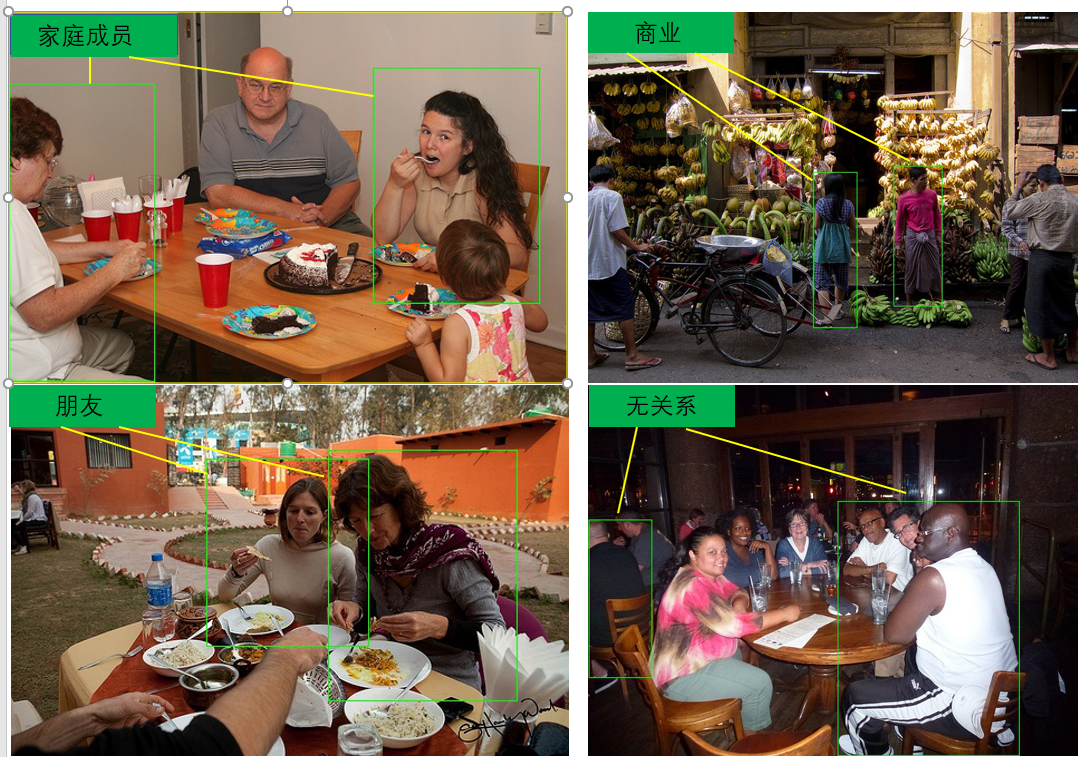
\includegraphics[width=0.95 \textwidth,clip]{example-1.png}
	%\hspace{0.02\textwidth}
	%\vspace*{-0.08cm}
    \caption{PISC数据集中的一些图片例子}
	\vspace*{-3.5mm}
	\label{fig:intro-example}
\end{figure}
\looseness=-1

既然社会关系理解对于理提升上述任务的关键资源,那么自然而然的,如何准确的理解社会关系成为需要研究者需要攻克的课题。一方面,一张图片的社会关系可以通过众包的方式,人工标注得到,比如现有的数据集PISC\cite{li2017dual-glance}和PISC-relation\cite{sun2017a}。当然,自动端到端的方法包括基于人脸特征、年龄、人的头部特征等特征信息的\cite{sun2017a,zhang2015learning}。还有利用周边环境的信息的模型\cite{li2017dual-glance,wang2018deep},这些模型通常需要一个物体检测器或者检测器中RPN(region proposal network),这都是需要引入额外的标注框或者预训练模型。也有通过对周边物体和社会关系共现的统计,例如``computer''和``professional''共同出现的概率较大,如果识别出存在``computer'',那么当前的关系很大概率是``professional'',通过神经网络引入这些先验知识来提升预测的准确率。这些自动识别社会关系的模型虽然不断在进步,但是从实验结果来看,他们与人工标注的准确率还是存在很大鸿沟,离实际的应用还存在很大的距离。

然后,现有的学习模型大都倾向于利用外部的知识来辅助理解图片的社会关系场景,但是得到这些外部知识需要额外的人工标注,这是一件耗时耗力的工作,或者一些统计得到的先验知识同样包含一些噪音,这也直接引出了到底是否应该引入外部知识,例如是否利用周边物体的信息,以及如何在缺乏这些信息的情况下取得好的实验效果。受到场景图谱生成的启发,场景图谱的概念最初是在2015年由Johnson 等人\cite{johnson2015image}提出的,是用于描述图片的一种新的半结构化的方式,基本组成单位是视觉三元组,形式为(头实体,关系,尾实体)。受到该领域下xu(2017)\cite{xu2017scene}的工作首先将整张图片输入,考虑到图片中不同视觉三元组之间的相互影响。例如,当知道``马在草地上''倾向于提高检测到``人骑着马''这条视觉三元组。对于社会关系检测的场景,如果图片中包含三个人对,其中两个人对的社会关系是``朋友'',那么第三条关系的的社会关系会倾向也是``朋友''或者其他的亲密关系,而不是``无关系''。直观上来说,这个是成立的,因此我们可以利用这当前场景下的其他的关系的来推理出当前的关系。

本论文主要研究如何将前文提到的关系场景的上下文信息引入社会关系理解的框架中。本文的出发点完全区别于Li(2017)\cite{li2017dual-glance}和Wang(2018)\cite{wang2018deep}的工作,
,对于关系特征的提取方法采用和Li\cite{li2017dual-glance}相同的策略。论文的切入点如图例\ref{fig:intro-example-2},图上六个人对的关系有五对是``朋友''关系,其中只有一对``奶奶-孙女''的关系,因此当前的图片应该是一个朋友聚会的场景拍下的。如果我们想推理出其中一个人对的关系并且已经知道其他部分人对的关系,那么直观的,我们会通过对已经知道的关系进行一个场景的判断,从而推理当前人对的关系到底是什么。在当前例子中,如果已经知道了2对或者3对都是``朋友''关系,那么当前的人对大概率也是``朋友''关系。因此,类似于前文提到的场景图谱的生成,以及现有的社会关系理解的研究现状,将当前的工作成为社会关系图谱生成
(social graph generation)。
\begin{figure}[htpb]
	\centering
	%	\includegraphics[width=0.48 \textwidth, trim=10 10 10 80,clip]{./pic/example_new.pdf}
	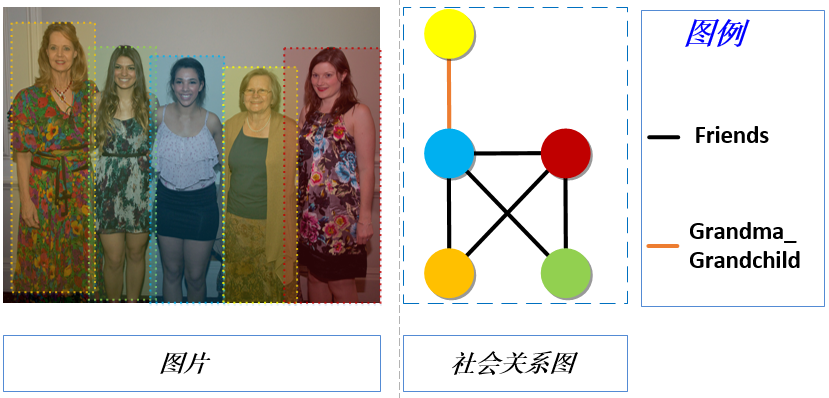
\includegraphics[width=0.95 \textwidth,clip]{example-2.png}
	%\hspace{0.02\textwidth}
	%\vspace*{-0.08cm}
    \caption{本论文动机的示例图,该图片来自PIPA-relation数据集,其中图片中对应阴影颜色的人对应社会关系图的部分,图上节点间的边表示他们之间的社会关系}
	\vspace*{-3.5mm}
	\label{fig:intro-example-2}
\end{figure}
\looseness=-1

在上述的介绍中,我们分别提到了两方面的相关内容,一方面社会关系理解的意义和作用,另外提到了与社会关系同属视觉理解领域的场景图谱的生成,收到这些工作的影响,可以列出他们的共性和特性如下:
\begin{enumerate}
    \item 场景图谱的基本组成是视觉三元组,社会关系图中是人对和人对间的社会关系,但是场景图谱中并没有人的的类别的概念,社会关系图中节点间的社会关系与人的类别无关。
    \item 场景图谱中的关系类别较多,有80-100个类别,但是在社会关系中,现有数据集不同粒度的关系类别分别为3、6、16,数量上远远不一样。并且在场景图谱中,关系的类型主要以空间关系为主,少量含有语义的关系,但是在社会关系图中,除了``无关系''和空间存在较大关联,其他的均为语义的关系。
    \item 与现有研究工作的区别是,之前的方法均将同一张图片上的不同人之间的关系割裂来看,但是他们间的关系互相影响,现有的研究工作忽略了这一点。
\end{enumerate}

要想解决社会关系理解问题,一种可行的方法是借助场景中除了人以外其他的信息,由于现有的数据集并没有标注其中的物体信息,所以需要借助额外的检测模型,但是由于模型的准确率的原因,会引入相当一部分的噪音,我们不能简单的加入这些信息,或者说我们是否需要加入这部分信息。其次是借助场景图谱生成的思想,认为一张图片中所有人对的社会关系不是割裂开的,是一同生成的,并且它们之间是相互影响的,但是由于场景图谱和社会关系图的区别,我们需要设计一个在社会关系理解人物下人对关系之间的交互机制。

\section{研究现状}

\subsection{视觉关系理解的应用}
在计算机视觉领域,社会关系信息被探索来提升几个常见的任务,例如人的轨迹预测\cite{kim2015brvo,robicquet2016learning}、 多目标追踪\cite{chen2012discovering,qin2012improving}和群体活动识别
\cite{direkoglu2012team,lan2012social,lan2012discriminative}。例如,在Deng等人(\cite{deng2016structure})群体活动识别的任务中,群体活动识别需要推理出图上人之间的结构信息,当前的方法是判断每个个体的动作,并且判断图上人之间的关系。但是由于图片特征的复杂和不确定性,这两个任务都是很有挑战的,推断出图上的结构信息能帮助排除一些未参与群体活动的人,得到更好的预测结果。因此预测这些人之间的社会关系能有助于群体活动识别。如图例\ref{fig:deng-example}所示,利用深度学习模型得到的人的表征和场景的表征后,如果知道了图例中第三个人和另外两个人之间不存在关系的情况下,排除第三个人对任务判断的影响。能更为容易的得出当前的群体活动场景是``waiting''。如Alahi(2016)\cite{alahi2016social}、robicquet等人(2016)\cite{robicquet2016learning}隐含的引入了社会性的约束来预测符合社会常识规则的人类运动轨迹,利用LSTM网络在序列任务的优越性,同时设计了特殊的池化模块来考虑邻居的运动走向。但是可以通过加入已经识别好的社会关系,即人与人之间的相互作用,当作常识规则来增强对运动轨迹预测鲁棒性和准确率。
\begin{figure}[htpb]
	\centering
	%	\includegraphics[width=0.48 \textwidth, trim=10 10 10 80,clip]{./pic/example_new.pdf}
	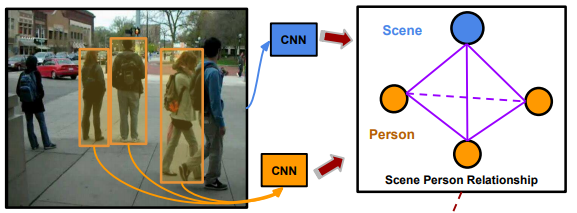
\includegraphics[width=0.95 \textwidth,clip]{deng-example.png}
	%\hspace{0.02\textwidth}
	%\vspace*{-0.08cm}
    \caption{来自Deng等人\cite{deng2016structure}的示例图}
	\vspace*{-3.5mm}
	\label{fig:deng-example}
\end{figure}
\looseness=-1

在社会关系理解之外,也有很多的工作明确的关注社会属性和社会结构的识别Wang等人(2010)\cite{wang2010seeing}通过分析个人的相册集来实现个人的家庭社会关系识别,
亲属关系验证\cite{dibeklioglu2013like,fang2010towards,xia2012understanding}和亲属识别\cite{chen2012discovering,guo2014graph}等任务也被广泛的探索和研究。Zhang等人(2015)\cite{zhang2015learning}研究人的面部表情,例如友好的、统治的,这些信息有助于推断社会关系。而在基于视频分析的领域中,Ding等人\cite{ding2014learning}从电影中挖掘演员的关系。社会关系理解在某个方面和社会信号处理\cite{vinciarelli2009social},社会信号处理的目标是利用多个传感器理解社会信号和社会行为,例如角色识别、影响力排名和统治力检测等\cite{hung2007using,rienks2006detection,salamin2009automatic}。但是本文关注的社会关系理解本质上不同于前面提到的这些工作,和基于面部表情的社会关系检测不同的是,本文的研究图片中的个体往往是姿态和朝向都不确定的。此外,本文着重的社会关系是更普遍的社会关系,而不是家庭相册中的亲属关系。与视频任务不同的是,本文关注的一张图片中的视觉信息。

前面的社会关系理解的工作大多数都是利用向量化的社会关系来帮助推理,与社会关系理解同属同一个视觉关系理解任务类别,即场景图谱的生成,又或者称为视觉关系检测。该任务的最早是Johnson等人于2015年提出的
\cite{johnson2015image},是一种用于描述图片场景的新的方式,与本文工作不同的是,场景图谱中的主要组成部分不仅包括人,还包括很多日常物体,如图\ref{sg-example}所示。两个工作最核心的挑战在于推理出物体之间的关系。由于场景图谱常用于图片检索\cite{johnson2015image},Marino(2017)\cite{marino2017the}利用得到场景图谱结合图神经网络提高图片的分类效果。在以上关于视觉信息理解的两个方向上,都有大量的工作提出,分别用于解决不同场景的问题,因此如何更好的实现视觉理解这个难题自然而然的成为许多研究者想要攻克的难题。对于场景图谱来说,本文的工作主要受到了以下几个工作的启发。Xu等人(2017)对于场景图谱进行建模,分别包含物体节点和关系节点,然后采用Message Passing的方式进行迭代。通过相邻的节点或边对目标节点或边进行约束,从而对这些特征进行微调,达到提升的效果。Yang等人(2018)利用图卷积网络进行不同节点之间的Message passing来达到约束的效果。融合自然语言知识提出的VRD模型\cite{liang2018visual},本文初始步骤中的特征提取工作中包含空间信息的提取便收到该工作的启发。
\begin{figure}[htpb]
	\centering
	%	\includegraphics[width=0.48 \textwidth, trim=10 10 10 80,clip]{./pic/example_new.pdf}
	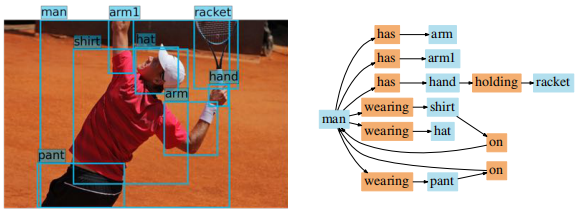
\includegraphics[width=0.95 \textwidth,clip]{sg.png}
	%\hspace{0.02\textwidth}
	%\vspace*{-0.08cm}
    \caption{场景图谱\cite{xu2017scene}的示例图}
	\vspace*{-3.5mm}
	\label{fig:sg-example}
\end{figure}
\looseness=-1

\subsection{社会关系理解的方法}
而对于社会关系理解,作为最早的工作,wang等人(2010)开始引入家庭关系当前背景来识别人之间亲属关系。在后来的工作中\cite{dibeklioglu2013like,xia2012understanding,chen2012discovering},为了捕获这些社会关系展现出来的一些规律,探索了面部表情和属性等用于亲属关系识别和验证。并且为了促进社会关系理解领域的研究和发展,Li\cite{li2017dual-glance}和Sun\cite{sun2017a}构建了大规模的数据集,并且利用深度学习的模型直接从图片中学习来识别关系。对于Sun构建的数据集PIPA-Relation,该数据集的关系包括5个领域,然后基于这5个领域又划分为16条关系。同样,Li基于关系模型理论,定义了一系列的关系列别,包含两个不同层次关系的划分,粗粒度的3类关系和细粒度的6类关系。在Sun(2017)等人的工作中,不仅提出了两个关系粒度的数据集,而且提出了Dual-glance模型。该模型是一个流水线的模型,并且包括两个模块,主要的的创新点在于利用人对周边的物体信息来提升关系检测的效果。Wang(2018)等人提出了基于知识图谱的深度推理模型,通过图门控神经网络引入物体的社会关系的共现的常识知识来实现物体和关系之间的推理,本质上还是利用周边的物体信息,但是在Dual-glance中,用到只是周边的物体区域,并不需要准确的识别出物体区域的物体类别。

在关系理解领域,除了社会关系理解,还有视觉关系检测任务。与社会关系检测不同,视觉关系检测首先依赖于一个物体检测器识别出所有的物体,然后依次两两识别两个物体存在的关系。在社会关系检测中,物体的类别只有人,并且一张图片中的人往往不会太多。Lu等人\cite{lu2016visual} 提出首先提出VRD 模型,利用自然语言得到的词向量作为先验知识来帮助单条三元组的检测。后来,Zhang 等人\cite{zhang2017visual} 提出VTranE 模型,模拟知识图谱中关系翻译,即$h + r = t$,本质上还是一个关系的分类器。但是并没有考虑到视觉关系的复杂度,并且不同于自然语言的状态翻译。Li (2017)等人\cite{li2017scene}进一步提出了多任务混合模型,任务包括场景图谱、区域描述生成、物体识别。和VRD类似,通过多种任务联合训练,引入额外的信息。Zellers 等人(2018)\cite{zellers2018neural}提出motif-net,通过分析数据集得出关视觉关系严重依赖头尾实体的类别,利用双向循环神经网络对物体类别编码信息进行编码处理,提升了物体识别的准确度,进而提升了任务的效果。

\subsection{研究现状小结}
当前社会关系理解领域的工作主要方式是引入额外的信息,例如引入面部表情和属性、年龄等。以及通过物体检测的方法识别出当前场景中的物体,来优化单纯通过提取人的区域的表征。最新的工作尝试引常识知识,对物体和关系间的常识知识进行表征来提高模型的效果。无论是采用额外的物体检测模型还是通过引入常识知识,都是外部信息,不可避免的需要额外的消耗或引入一些噪声。同时,对于人的轨迹预测、 多目标追踪 和群体活动识别任务,引入社会关系的信息能有效的提高这些任务的效果。因此,如何利用更少的信息,来提升预测效果是当前的一大挑战。同时以消息传递机制为技术栈的微调机制的方法在场景图谱,同属视觉理解领域得到了运用,在一定程度上解决了场景图谱的生成问题。然而,由于场景图谱和社会关系任务理解两个不同人物上的区别,如何在社会关系理解中引入消息传递机制仍然面临很多的挑战

\section{本文工作}

本文首先通过介绍现有的社会关系理解最新研究工作,分析它们的模型设计的出发点,模型的结构,分析这些工作的忽略的信息,即没考虑到整张图片不同的人对的关系之间的互相影响。因此,本文提出了一个考虑到同一张图片不同关系之间存在交互的模型:包含人对消息传递机制的模型,人对关系网络(Person-pair Relation Network),简称PPRN,最后把该模型应用到社会关系理解的任务中,在两个公开数据集上做了对比实验。
本文提出的PPRN模型包括以下模块:
\begin{enumerate}
    \item 特征抽取模块,对于特征抽取模块,本文采用一个ResNet101\cite{he2016deep}抽取两个人的单独区域的特征,同时另外一个ResNet101抽取人对区域的特征。同时,对于这个模块,人对的位置信息也加入了最后的表征向量中。
    \item 消息传递模块,本文首次尝试在社会关系理解任务中引入多个人对之间的关系的想法。对于消息传递模块,利用以GRU单元为组件的RNN来实现消息传递,并且设置多个迭代步,实现消息传递和池化模块的交互。采用RNN 最后隐藏层的输出作为图片中人对的关系表征。
    \item 消息池化模块,本文设计了一个交互机制来处理人对之前的关系的信息,同时利用注意力机制来提高模型的表现效果。
    \item 融合周边物体信息模块,与Dual-galnce\cite{li2017dual-glance}类似,本文在经过消息传递、池化两个模块后得到的人对关系编码,利用注意力机制得到周边物体区域特征编码。两部分特征融合后,进行最后的关系分类。
\end{enumerate}
在实验中,本文在两个公开数据集上验证了\textbf{PPRN}模型的有效性,它们分别是PIPA-Relation和PISC,其中PISC包括两个粒度的子数据集PISC-coarse和PISC-fine。与此同时,在加入最后的周边物体信息模块后,模型效果轻微下降。
接着,本文进一步通过案例研究的方法分析了\textbf{PPRN} 模型的具体效果。从实验结果可以看出,\textbf{PPRN}模型在与其他基准模型的比较中取得了在两个数据集上取得了最优的结果,说明了引入不同关系之间交互的消息传递机制在社会关系理解为基础场景中的重要性。

\section{论文结构}

全文的组织结构描述如下:

第1章:介绍了社会关系理解的相关背景,点明了当前社会关系理解存在的缺点,由此引入了同属视觉关系理解人物的场景图谱,分析并总结了场景图谱的研究现状,并针对两者的共同点引出社会关系理解的提升方案。

第2章:首先介绍了图像领域的视觉信息抽取的方法,从简单的神经网络、卷积神经网络、以及残差网络等介绍。之后基于前面的神经网络的知识,介绍了现有工作中常用的物体检测与识别的方法,并进行了讨论与对比。然后详细介绍了当前社会关系理解模型的各个部件,最后对本章内容进行了总结。

第3章:针对社会关系理解的特点,提出了基于消息传递机制的社会关系理解方法,设计了图像中不同人对的社会关系交互的PPRN模型,并且具体介绍了模型的细节。同时实现了结合周边物体信息的模块,分析了模型的设计原则和具体细节。

第4章:首先介绍了两个在社会关系理解领域常用的数据集,并对PPRN模型在不同关系粒度的数据集上进行了训练和测试,接着针对实验结果进行了分析。然后还进一步通过案例研究的方式分析了PPRN在社会关系理解的变现。

第5章:总结了本文的研究工作,并且提出了进一步的研究展望。




%\clearpage{\pagestyle{empty}\cleardoublepage}       %本有
% !Mode:: "TeX:UTF-8"

\chapter{预备知识}
\label{ch:pre}



\section{图像的视觉信息抽取}


\subsection{一般神经网络}
神经网络(neural network)的方面的研究就出现了,早起的神经网络主要是指生物学中的``生物神经网络'',在当前计算机领域特指``神经网络学习''。神经网络最基本的结构是神经元模型,神经元模型如图\ref{fig:nn-example},在这个模型中包括输入端、神经元权重(weight)、偏差(bias)、激活函数(activation function)、阀值、输出。在这个模型中,当前神经元接收其它$n$个神经元的输入,与连接权重相乘之后加上偏差,然后激活函数的处理得到激活值输出。
\begin{figure}[htpb]
	\centering
	%	\includegraphics[width=0.48 \textwidth, trim=10 10 10 80,clip]{./pic/example_new.pdf}
	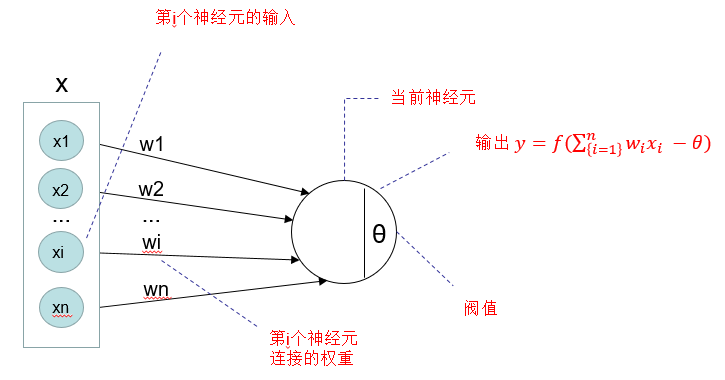
\includegraphics[width=0.95 \textwidth,clip]{nn.png}
	%\hspace{0.02\textwidth}
	%\vspace*{-0.08cm}
    \caption{神经元模型示意图}
	\vspace*{-3.5mm}
	\label{fig:nn-example}
\end{figure}
理想中的激活函数是如公式\ref{eq:activate-sgn},将输入值映射为输出值"1"或者"0",其中"1"对应神经元兴奋,"0"对应于神经元抑制,但是因为该阶跃函数具有不连续、不光滑等性质。因此常采用Sigmoid函数作为激活函数,一般来说激活函数是非线性的、可微的。如果不使用线性激活函数,采用线性激活函数(恒等激活函数,图例中$f(x) = x$)的话,那么神经网络只是把输入线性组合再输出,和没有采用神经网络是一样的。
\begin{equation}\label{eq:activate-sgn}
    sgn(x)=\left\{
    \begin{aligned}
    1, x\geq 0 \\
    0, x<0 \\
    \end{aligned}
    \right.
\end{equation}
例如sigmoid函数可以把$(-\infty,+\infty)$输入值映射到(0,1)区间内。常见的激活函数还有tanh(hyperbolic tangent, tanh)函数、修正线性单元(rectified linear units,ReLU)函数等等。表\ref{tab:activate-func}详细的列出了3个常用激活函数的原函数、一阶导数、以及函数的值域。其中tanh函数只是sigmoid函数向下平移再拉升的结果。并且在实际应用中,tanh的效果是好于sigmoid,因为tanh的函数值域是属于(-1,1)的,使用tanh代替sigmoid,会使得神经元输出的均值趋近于0而不是0.5,这样的结果会使得下一层的学习变得更加简单。但是对于多层的神经网络,sigmoid和tanh在极大或极小时梯度会趋近于0,会造成梯度弥散问题。但是对于ReLU 来说,当小于0时,梯度是小于0的,当大于0是,梯度是常数。ReLU激活函数在实际训练中取得了良好的效果。但是对于小于0的部分,此时的梯度为0,神经元不会训练,因此研究者们提出了LeakyReLU等激活函数解决这一问题。
\begin{table}[htpb]
  \centering
  \caption{常见激活函数的介绍}
  \label{tab:activate-func}
  \begin{tabular}{c|c}
    \toprule
    函数名称~~~ & 原函数 ~~~~~~~~一阶导数$f^{'}(x)$~~~~~~~~原函数值域 \\
    \midrule
    sigmoid函数 & $\sigma(x) = \frac{1}{1+e^{-x}}$ ~~~~~~~ $f^{x}(x)=\sigma(x)(1-\sigma(x))$ ~~~~~~~ (0,1) \\ \\
    tanh函数 & $tanh(x) = \frac{e^x-e^{-x}}{e^x+e^{-x}}$ ~~~~ $f^{'}(x)=1-tanh(x)^{2}$ ~~~~ (-1,1) \\ \\
    ReLU函数 & $relu(x) = max(0,x)$ ~~~~~~~~  $sgn(x)=\left\{ \begin{aligned} 1, x\geq 0 \\ 0, x<0 \\ \end{aligned} \right.$ ~~~~~~~ $ [0,+\infty)$ \\ \\
    \bottomrule
  \end{tabular}
\end{table}

前面介绍了神经元模型和各类激活函数,这里需要提到是深度神经网络、目标函数、优化方法。相比前面的单层神经网络,更常见的如图\ref{fig:mnn-example}所示的包含多个层级结构的神经网络,又称为``多层前馈神经网络''(multi-layer feed forward neural networks),其中神经元同一层之间不存在连接,跨层的神经元之间也不存在连接。就如图\ref{fig:mnn-example}所示,其中输入层的神经元接收外接的输入,隐层与输出层的神经元对输入的数据进行处理,这里的网络包含两个隐藏层(hidden layer)和一个输出层(output layer),假设输入为$x$,那么该网络可以形似化为
$H_{\theta}(x) = f_3(w_{3}f_2(w_{2}(f_{1}(w_{1}x+b_1))+b_2)+b_3)$, 其中$f_{1},f_{2}$分别是隐藏层的激活函数,$f_{3}$是输出层的激活函数。假设对于当前任务的目标函数(object function)如\ref{eq:loss-1},需要最小化目标函数$L_{\mathbf{X},\mathbf{Y}}$的值, 对于训练的过程来说,就是不断接受输入层的$(x,y)$,$y$是样本的标签,随着$x$的不断输入,不断调整网络的连接权重$w_1,w_2,w_3$。 常用的优化算法包括随机梯度下降法(stochastic gradient descent,SGD)来迭代优化连接权重,对于一条样本$x_{i},y_{i}$,其连接权重的更新方法如。
\begin{equation}
    \begin{split}
        w_i  \leftarrow w_i +\bigtriangleup w
    \end{split}
\end{equation}
不同层之间的梯度通过误差逆传播(error Back Propagation 简称BP)\cite{rumelhart1988learning}算法进行整个网络的学习。SGD因为更新比较频繁会造成损失函数动荡,最终停留在局部最小值或鞍点。之后又新衍生出的包括Monmentum、Adagrad\cite{duchi2011adaptive}和Adam\cite{kingma2014adam},这些算法能减少迭代的轮数,训练速度更快的收敛到最优值。
\begin{equation}\label{eq:loss-1}
    L(\mathbf{X},\mathbf{Y}) = \sum_{(x_i,y_i) \in (\mathbf{X},\mathbf{Y})}(y_{i} - H_{x}(x_{i}))
\end{equation}

\begin{figure}[htpb]
	\centering
	%	\includegraphics[width=0.48 \textwidth, trim=10 10 10 80,clip]{./pic/example_new.pdf}
	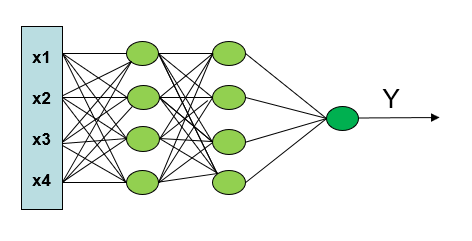
\includegraphics[width=0.80 \textwidth,clip]{multilayer.png}
	%\hspace{0.02\textwidth}
	%\vspace*{-0.08cm}
    \caption{两个隐藏层的神经网络示意图}
	\vspace*{-3.5mm}
	\label{fig:mnn-example}
\end{figure}

%%%%%%%%%%%%%%%%%%%%%%%%%%%   卷积神经网络的介绍   %%%%%%%%%%%%%%%%%%%%%%

\subsection{卷积神经网络的介绍}
卷积神经网络(Convolutional Neural Network,CNN)是深度学习的代表算法之一,由LeCun首次实现并且应用。卷积神经网络的主要作用是提取特征,该网络受到生物学的影响,相比较与全连接神经网络,卷积神经网络的主要特性包括局部感知和参数共享。局部感知指对于具有空间特征的输入来说,每个神经元没必要知道全局的信息,只需要感知局部的信息,然后在更高层将局部的信息合并起来得到更高层的信息。对于权值共享来说,每个卷积核与位置无关,因为假设对于图像来说,其中某一部分的统计特性和其它的部分是一样的,所以对于其中的一个卷积核来说,可以应用到图像上的任何地方去。所以,局部感知和参数共享不仅能提取到更多的特征,并且能大幅度减少参数的数量。因此,卷积神经网络广泛的应用在图像、视频、音频和文本等各种模态的数据上,并且都取得了巨大的成功。

卷积神经网络的特征提取层主要包括两个模块,分别是卷积层(convolutional layer)和池化层(pooling layer),两者的顺序,一般是先通过卷积层,然后是池化层。对于卷积层,主要的作用是提取特征,卷积层的核心是卷积核(kernel),其本质还是神经元。但是卷积核的感受野和全连接的神经元是不同的,这里的感受野是局部的,并且感受野的大小由卷积核的大小控制。如图\ref{fig:con-example}所示,当前卷积核的大小是$4 \times 4$的,对于输入的图片$6 \times 6 \times 3$,其中图片输入的3为图片的通道数、$6 \times 6$为高宽,假设滑动的步骤为$1$,卷积核通过在输入图片上按照步长进行滑动并且进行对应位置的点乘运算,最后形成一个$4 \times 4$ 的特征图。以上综合起来就是卷积操作,其中$3 \times 3$就是网络的参数。按照惯例,输入的图片可以有固定的的高宽和通道数时,卷积核可以有不同的高宽,但是必须是固定的通道数,这里一般和输入的通道数一致。有多少个卷积核,最后就能得到多少个特征图(feature map)。
\begin{figure}[htpb]
	\centering
	%	\includegraphics[width=0.48 \textwidth, trim=10 10 10 80,clip]{./pic/example_new.pdf}
	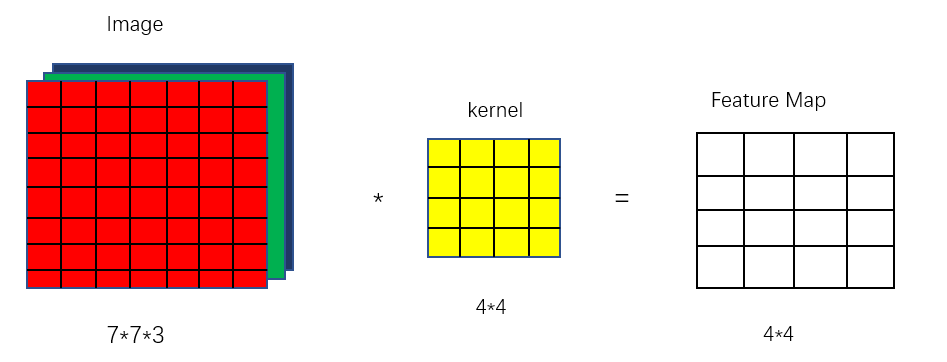
\includegraphics[width=0.95 \textwidth,clip]{conv.png}
	%\hspace{0.02\textwidth}
	%\vspace*{-0.08cm}
    \caption{卷积神经网络的卷积层示意图}
	\vspace*{-3.5mm}
	\label{fig:conv-example}
\end{figure}

对于池化层来说,主要的作用是对于卷积层输出的特征图提取主要特征,降低网络的参数,且有防止过拟合的作用。常见的池化包括平均池化(Average pooling)和和最大池化(Max pooling)。具体细节如图\ref{fig:pooling-example}所示,池化也是通过类似卷积的操作实现的,在图例中,池化也是以$2 \times 2$在特征图上进行滑动,滑动的步骤为$2$,而最大池化是选着窗口中的最大值作为输出,平均池化是选择窗口中所有值的平均值进行输出,假设输入的特征图为$C \times W \times H$ ,那么经过如图例所示的操作后得到的特征图为$C \times \frac{W}{2} \times \frac{H}{2}$。
\begin{figure}[htpb]
	\centering
	%	\includegraphics[width=0.48 \textwidth, trim=10 10 10 80,clip]{./pic/example_new.pdf}
	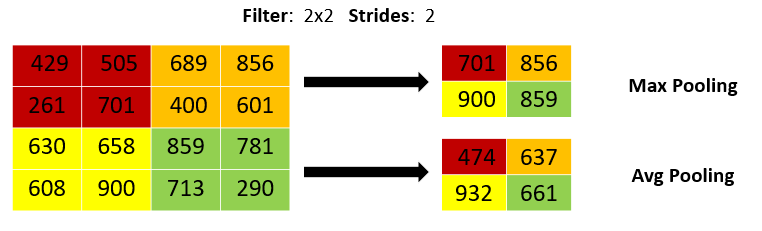
\includegraphics[width=0.95 \textwidth,clip]{pooling.png}
	%\hspace{0.02\textwidth}
	%\vspace*{-0.08cm}
    \caption{卷积神经网络的池化层示意图}
	\vspace*{-3.5mm}
	\label{fig:pooling-example}
\end{figure}

综合上述对于卷积神经网络的卷积和池化的介绍,因为每层的输入和输出都表现为特征图的形式,因此卷积神经网络可以和全连接的网络一样可以有多层,并且取得更好的效果。LeNet-5\cite{lecun1998gradient-based}是
Yang LeCun等人在$1988$年提出的,它是第一个成功应用于数字识别问题的卷积神经网络,在著名的MINIST数据集上,LeNet-5可以取得大约$99.2\%$的准确率。LeNet-5是一个经典的卷积神经网络,前5层分别是卷积层和池化层,后2层全连接层。之后于$2012$ 年提出的AlexNet\cite{krizhevsky2012imagenet},其网络结构如图\ref{fig:alexnet-example}首次使用Relu激活函数替代Sigmoid,并且验证了其在较深网络上的作用,成功解决了Sigmoid在较深网络的梯度弥散问题,虽然Relu 很早就提出了。其次,AlexNet首次在训练中使用dropout层抑制一部分激活的神经元,以避免过拟合,并且通过实践证明了效果。与此同时,模型还采用了数据增强等trick来防止过拟合,使用cuda提高训练速度。而之后提出的VGG\cite{simonyan2015very},相比较与之前的LeNet和AlexNet,最大的特点是网络更深,具有16-19层,不包含池化和最后的softmax层。
\begin{figure}[htpb]
	\centering
	%	\includegraphics[width=0.48 \textwidth, trim=10 10 10 80,clip]{./pic/example_new.pdf}
	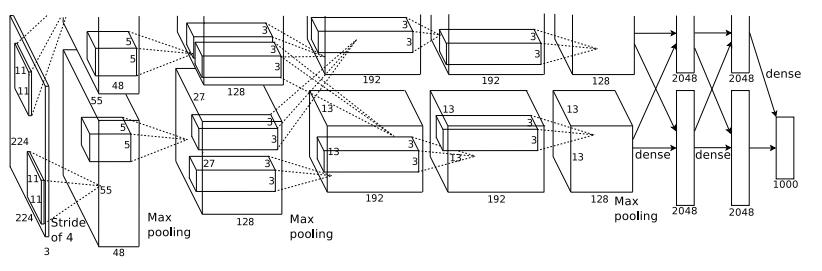
\includegraphics[width=0.95 \textwidth,clip]{alexnet.png}
	%\hspace{0.02\textwidth}
	%\vspace*{-0.08cm}
    \caption{AlexNet网络结构示意图}
	\vspace*{-3.5mm}
	\label{fig:alexnet-example}
\end{figure}
ResNet\cite{he2016deep}是何凯明等人(2016)提出的,针对前面网络并不能随着层数的叠加而性能的提高,ResNet首次提出了残差学习单元。如图\ref{fig:resnet-example}所示,假设模块的输入为$x$,$F(x)$指的是网络中的一系列的张量运算,假设神经网络最优的拟合结果为$H(x) = F(x) + x$,那么神经网络的最优的映射函数$F(x)$为$H(x)$和$x$之间的残差。通过不断的叠加这个模块,可以不断堆叠加深网络的深度但是不降低网络性能。
\begin{figure}[htpb]
	\centering
	%	\includegraphics[width=0.48 \textwidth, trim=10 10 10 80,clip]{./pic/example_new.pdf}
	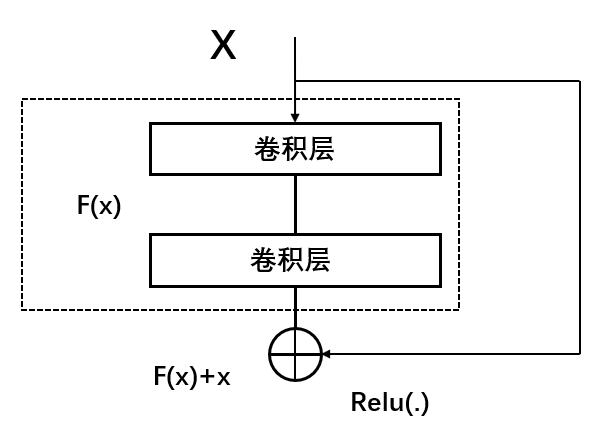
\includegraphics[width=0.75 \textwidth,clip]{resnet.png}
	%\hspace{0.02\textwidth}
	%\vspace*{-0.08cm}
    \caption{ResNet残差学习单元示意图}
	\vspace*{-3.5mm}
	\label{fig:resnet-example}
\end{figure}

综上,卷积神经网络自提出以来,得到了极大的发展,表现为新的激活函数,降低过拟合的dropout层,残差学习模块,加上cuda硬件加速的发展,我们能训练更复杂更深的神经网络,取得更好的性能。

%%%%%%%%%%%%%%%%%%%%%%%%%%%%%%%% 图推理 %%%%%%%%%%%%%%%%%%%%%%%%%%%%%%%%%%%%%%%%%%

\subsection{消息传递}

图推理是消息传递的一种形式,条件随机场(Conditional Random Field)广泛的用在了图推理问题上。Johnson\cite{johnson2015image}将CRF用于图像检索领域的场景图谱与对应图片的绑定的推断。本文用的方法类似于CRFasRNN\cite{zheng2015conditional}和Graph-LSTM\cite{liang2016semantic}。本文的方法是收到\cite{xu2017scene}的启发,Xu在场景图谱的生成任务中,设计了原始图和对偶图,原始图用于图片中物体节点的预测,对偶图用于关系节点的预测。和之前不同的是,我们只是对其中的关系节点构建图,通过关系的消息传播机制,我们的模型是迭代的提纯社会关系理解的预测。而不是像标准的循环神经网络(Recurrent Neural Network)只是单次预测,并不能达到提纯的效果。下面的部分我们介绍关于CRF和本文中用到了循环神经网络(RNN)以及门控循环网络(Gated Recurrent Unit,GRU)。

\subsubsection{条件随机场}
CRF是一种判别式无向图模型,用于对条件分布建模,在给定随机变量\textbf{X}的条件下,构建条件概率模型\textbf{P(Y|X)}。条件随机场的定义如下:设\textbf{X}与\textbf{Y}是随机变量,\textbf{P(Y|X)}是在给定
\textbf{X}的条件下\textbf{Y}的条件概率分布。令G = (V,E)表示一个无向图,V是节点的集合,E是无向边,$Y_{v}$表示与节点v对应的标记向量,$w~v$表示在图中所有与节点v有边连接的所有节点w,
$w \neq v$表示节点v以外的所有节点,如果所有的节点$Y_v$都满足公式\ref{eq-crf}  的马尔科夫性质,那么称(Y,X)为一个条件随机场。
\begin{equation} \label{eq-crf}
    P(~Y_{v}~|~X,Y_w,w \neq v~) = P(~Y_v~|~X,Y_w,w~v~)
\end{equation}
CRF引入了特征函数(指数函数的形式),对于其中的特例线性链条件随机场,线性链条件随机场如图\ref{fig:crf}。
\begin{figure}[htpb]
	\centering
	%	\includegraphics[width=0.48 \textwidth, trim=10 10 10 80,clip]{./pic/example_new.pdf}
	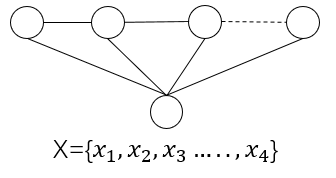
\includegraphics[width=0.75 \textwidth,clip]{crf.png}
	%\hspace{0.02\textwidth}
	%\vspace*{-0.08cm}
    \caption{线性链条件随机场}
	\vspace*{-3.5mm}
	\label{fig:crf}
\end{figure}
其中概率分布如下所示,其中$t_{k}$和$s_{l}$都是特征函数,$\lambda_{k}$和$\mu_{l}$对应的权值。
\begin{equation}
    P(y~|~x) = \frac{1}{Z}\mathbf{exp}((\sum_{i,k})\lambda_{k}t_{k}(y_{i-1},y_{i},x,i)+\sum_{i,l}\mu_{l}s_{l}(y_{i},x,i))
\end{equation}

\subsubsection{循环神经网路}

循环神经网络(RNN)是神经网络的一种,主要用于处理序列序列建模问题。其基本结构如图\ref{fig:rnn}所示,相比其他类型的网络,其就是对神经网络展开k个步骤,所有的输入共享一个网络模块\textbf{S}。假设其中的参数为$\mathbf{W}_s$和$\mathbf{W}_x$,那么所有模块的这个两个参数是共享的。对于标准的RNN结构,第t步,RNN的输出向量$\mathbf{s}_t$如公式\ref{eq:rnn}所示计算。
\begin{figure}[htpb]
	\centering
	%	\includegraphics[width=0.48 \textwidth, trim=10 10 10 80,clip]{./pic/example_new.pdf}
	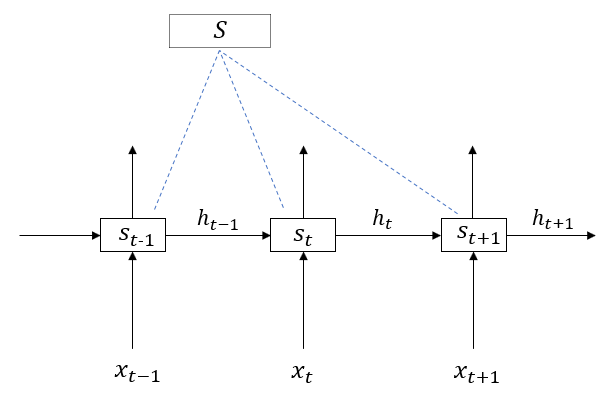
\includegraphics[width=0.75 \textwidth,clip]{rnn.png}
	%\hspace{0.02\textwidth}
	%\vspace*{-0.08cm}
    \caption{}
	\vspace*{-3.5mm}
	\label{fig:rnn}
\end{figure}
由于标准的RNN网络会由于结构的问题,无法处理梯度消失和梯度爆炸的问题。后续的研究人员对于其提出的梯度消失的问题,有LSTM\cite{hochreiter1997long}和GRU\cite{cho2014learning}等改良的RNN网络。这里着重介绍本文中用到的GRU结构。基本结构如图\ref{fig:gru},GRU解决梯度消失主要是引入了一个更新门(update gate),该机制可用于控制在BP算法时,计算梯度的时候,通过更新门记住之前的信息,使得求导时不会陷入极小的情况,从而达到解决梯度消失问题。
\begin{figure}[htpb]
	\centering
	%	\includegraphics[width=0.48 \textwidth, trim=10 10 10 80,clip]{./pic/example_new.pdf}
	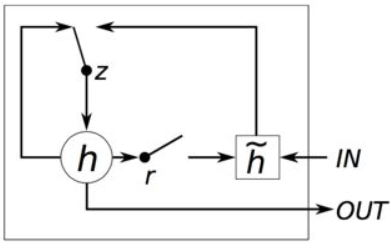
\includegraphics[width=0.5 \textwidth,clip]{gru.png}
	%\hspace{0.02\textwidth}
	%\vspace*{-0.08cm}
    \caption{}
	\vspace*{-3.5mm}
	\label{fig:gru}
\end{figure}

\begin{equation}\label{eq:rnn}
    s_t = \mathbf{tanh}(\mathbf{W}_s*h_{t-1}+\mathbf{W}_x*x_{t}+b)
\end{equation}


%%%%%%%%%%%%%%%%%%%%%%%  物体的检测与识别技术  %%%%%%%%%%%%%%%%%%%

\section{物体检测与识别}

在社会关系识别的任务中,有一个重要的模块是利用物体识别模型得到人的场景信息,即采用物体识别模型识别去当前图片中包含了哪些物体,得到该物体在图片的区域。物体识别的模型包括Ross等人提出的RCNN\cite{girshick2014rich},fast-RCNN\cite{girshick2015fast},以及Ren等人(2016)\cite{ren2015faster}提出的faster-RCNN。前面提到的三个模型都是基于区域的物体检测模型,RCNN\cite{girshick2014rich} 首次提出在目标图像中有多个目标框,然后判断目标框是否包含物体,具体的检测步骤如下:
(1)其中采用选择性搜索的方法得到图片中的所需要的目标框区域,将得到的区域调整为卷积神经网络输入的消息。
(2)利用一个预训练好的卷积神经网络,提取第一步得到的区域中的特征。
(3)将第二步中得到的特征当作一个线性SVM的输入,得到物体的类别,另外训练一个线性回归模型得到物体的目标框。
RCNN的主要缺点是对于一张图片中的每个感兴趣区域,需要遍历提取其中的特征,然后依次执行物体的分类和物体框的回归,需要耗费较多时间。由于全卷积和池化层不改变某个区域在特征图和原图的位置,因此fast-RCNN 在RCNN 的基础上提出了ROI(region of interest) 池化层,将图片输入到卷积神经网络中,对于特征图上的区域,经过ROI池化层进行调整,然后再继续之后的全连接层和一个线性回归层进行分类和目标框的确定。综上,fast-RCNN 较大程度上提高了物体检测的性能。由于fast-RCNN 在大数据集上的表现依然不能满足实际的需求,因为RCNN和fast-RCNN均采用选择性搜索的方法得到所需要的区域,这个步骤是比较耗费时间。因此faster-RCNN提出RPN(region proposal network),RPN主要网络包括两部分,一部分主要是对生成的anchors进行判断是foreground还是background,其中foreground代表目标,另外一部分主要是对检测框的位置进行调整。经过RPN网络后得到候选区域,再利用ROI池化得到特征向量进行物体类别的判断和物体框的进一步精确判断。

综上,以上的篇幅主要是回顾了在社会关系检测的工作中,有用的物体检测方法和一些相关工作。结论是得益于GPU等硬件设备的发展,物体识别领域的算法也得到了快速的发展,尤其是随着特征提取模块的发展,卷积网络越来越深,能学习到更多更丰富的特征。对于一幅图片,我们能在得到更多的、更准确的物体框和类别。

\section{社会关系检测}
本章将回顾社会关系检测领域的一些相关工作,并且对于消息传递机制的介绍,以及消息传递机制的相关工作的一些介绍。

\subsection{已有工作的简单介绍}

社会关系检测是社交网络的一个基础\cite{li2015celebritynet},社会关系检测作为一个重要的多学科问题,在计算机视觉领域受到越来越多的关注。随着这个问题被提出以来,有大量的工作用于从图片中抽取两个人之间的社会关系。主要有wang 等人(2010)\cite{wang2010seeing},以及Dibeklioglu等人(2013)\cite{dibeklioglu2013like}和Zhang 等人(2015)\cite{zhang2015learning}提出的利用面部表情、年龄、性别、姿势等多种特征的联合模型。Li等人(2017)\cite{li2017dual-glance}提出的多次观察的\textbf{dual-glance}模型。以及Wang 等人(2018)\cite{wang2018deep}提出的基于常识知识的深度推理模型\textbf{GRM}。以及从视频中抽取社会关系的工作ding等人(2010)\cite{ding2010learning}、Ramanathan等人 (2013)\cite{ramanathan2013social}。Sun等人(2017)\cite{sun2017a}基于范围的理论,将社会关系划分为5个范围,同时接着这五个范围又划分为16种社会关系并且扩充了PIPA(people in photo album)数据集\cite{zhang2015beyond},得到了PIPA-relation。

Zhang~等\cite{zhang2015learning}提出的模型认为从心理学的角度出发,认为人的关系主要由人的面部表情的一些特点决定的。首先,模型设计了一个基准模型用于提取图片中两个人对的特征,对于两个人对,基准模型采用共享参数的深度卷积网络(DCN),利用DCN提取得到的特征分别记为$\mathbf{x}^r,\mathbf{x}^l$,并且$\forall \mathbf{x}^r,\mathbf{x}^l \in R^{2048 \times 1}$,经过一个权重矩阵$\mathbf{W} \in R^{4096 \times 256}$ 得到特征向量$x_t$。 对于已经标注好的人脸图片两个人脸分别为和,利用DCN 提取得到的特征分别记为和,并且。除了图片中本来的特征,模型利用了两张人脸在图片的空间信息。1)两张人脸的位置分别表示为${x^l,y^l,w^l,h^l,x^r,y^r,w^r,h^r}$,其中$x-,y-$是左上角的坐标,$w,h$ 分别是两个人脸包围盒的宽度和高度。2)人脸的相对位置$\frac{x^l-x^r}{w^l},\frac{y^l-y^r}{h^l}$。3)人脸之间的比例$\frac{w^l}{w^r}$。以上的三项空间特征会和DCN得到的$\mathbf{x}_t$拼接来学习得到关系类别。
\begin{figure}[htpb]
	\centering
	%	\includegraphics[width=0.48 \textwidth, trim=10 10 10 80,clip]{./pic/example_new.pdf}
	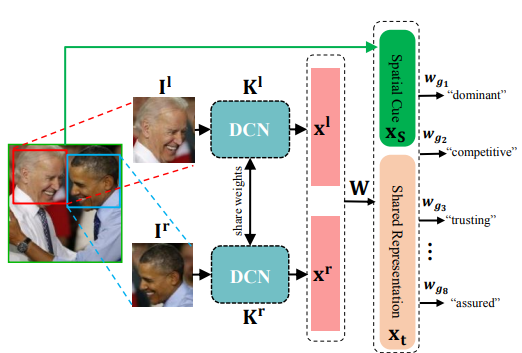
\includegraphics[width=0.75 \textwidth,clip]{1.png}
	%\hspace{0.02\textwidth}
	%\vspace*{-0.08cm}
    \caption{zhang的模型}
	\vspace*{-3.5mm}
	\label{fig:model_zhang}
\end{figure}
\looseness=-1
除此之外,$\mathbf{w_{g_{i}}}$,$\mathbf{W}$,$\mathbf{K}^l$,and $\mathbf{K}^r$可以采用标准的正太分布初始化。结合之前符号的定义,该模型损失函数定义如下:
\begin{equation}
\begin{split}
     arg\max \limits_{\Omega} p(\{\mathbf{w}_{g_{i}}\}_{i=1}^8, ~\mathbf{W}, ~\mathbf{K}^r & ~|~ \mathbf{g},~\mathbf{x_t},~\mathbf{x_s},~\mathbf{I}^r,~\mathbf{I}^l) \propto \\
     (\sum_{i=1}^{8}~p(g_i~|~x_t,x_s)~p(w_{g_i}))~ & ~(\sum_{j=1}{K}~p(k_j^l)~p(k_j^r))~p(\mathbf(W)), \\
     s.t. ~\mathbf{K}^r &= \mathbf{K}^l
\end{split}
\end{equation}
基于以上的工作,该模型同样认为人的面部属性对最终的关系预测可以起到关键的作用。

Li等人(2017)\cite{li2017dual-glance}基于之前的工作,针对社会关系理解的务提出了包含两个关系粒度的数据集,PISC-coarse和PISC-fine(2017)\cite{li2017dual-glance}。该工作首次提出利用图片中的场景来协助预测两个人之间的关系,场景具体表示为该图片中的物体。直观来说,如果一幅图片中包含电脑桌子等物体,那么大概率是``同事''关系。\textbf{dual-glance}模型分为两个模块,first glance和second glance,first glance 的输入为一张图片$\mathbf{I}$ 和两个人身体的包围盒。针对图片$\mathbf{I}$,首先修剪出3个小块,前两个小块分别覆盖住两个人,$p_1$和$p_2$,第三个小块覆盖两个人,表示为$p_{u}$。这三个小块的像素被修正为$224 \times 224$大小,作为后续三个CNNs 网络的输入,其中$p_1$和$p_2$ 的特征抽取网络是共享网络参数的。此外,包围盒的位置信息对于视觉信息是一种补充,例如亲密关系往往的离得比较近的,无关系的两个人对的包围盒离的较远。位置信息$\mathbf{g}$,经过预训练的ResNet\cite{he2016deep} 抽取得到表示人对关系的特征向量为$\mathbf{v}$,经过拼接和全连接网络后得到这个人对的特征向量$\mathbf{v}_{top}$。

对于second glance模块,模型利用faster-RCNN\cite{ren2015faster}中的RPN产生一系列的区域候选框$P_{I}$,这些候选框包含物体的概率大于超参数$m$。对于一个人对,我们从集合$P_{I}$ 中选择部分候选框$R(b1,b2;I)$,选择方式如\ref{eq:select-rp},其中函数$G(b1,b2)$表示两个包围盒的IOU,$\tau_{u}$是阀值。
\begin{equation}\label{eq:select-rp}
    R(b1,b2;I) = \{c \in P_{I} : max(G(c,b1),G(c,b2))<\tau_{u}\}
\end{equation}
利用faster-RCNN得到的特征图,采用ROI pooling抽取出固定长度的的向量物体特征向量$v \in R^{k}$。同时用$\{v_i|i=1, 2, .... N\}$作为$R_(v1,b2;I)$中的物体向量集合。然后依次采用公式\ref{eq:atten-1}方式将$\mathbf{v}_{top}$和物体的向量集合得到$h_i$。
\begin{equation}\label{eq:atten-1}
    h_i = v_i + w_{top} \otimes v_{top}
\end{equation}
之后采用attention的方式将$h_i$得到最终的得分$s_i$,具体细节如公式\ref{eq:atten-2}所示,其中attention的权重$a_{i} \in [0,1]$
\begin{equation} \label{eq:atten-2}
    \begin{split}
        a_{i} &= \frac{1}{1+exp(-(W_{h,a}h_{i}+b_{a}))} \\
        v^{att}_{i} &= a_{i}v_{i} \\
        s_{i} &= W_{s} v_{i}^{att} + b_{s}
    \end{split}
\end{equation}

\textbf{GRM}(2018)\cite{wang2018deep}同样认为引入当前人对的周边物体的信息对判断人对之间的社会关系是有帮助的,但是现有前面的模型忽略了周边物体的语义和这些物体以及社会关系的先验知识。除此之外,周边物体和社会关系的交互太过简化了。因此,GRM采用深度学习结合先验知识制定了一个图推理模型(Graph Reasoning Model)来实现社会关系检测任务。首先,GRM基于训练集中的样本构建了一个描述物体和社会关系共现的图谱。形式化来说,先验知识图谱表示为$\mathrm{G} = \{\mathrm{V},\mathrm{A}\}$,其中$\mathrm{V}$表示图上的节点集合,$\mathrm{A}$表示节点间的邻接矩阵。当前的图$\mathrm{G}$包含两种节点类型,一种节点表示社会关系,一种表示物体类别,针对当前图片场景构建的图的节点来说,采用相应图片对应区域抽取出的特征向量初始化。对于社会关系节点,这里采用Li等人的方式\cite{li2017dual-glance}的方式修剪出三部分包含人的区域,利用预训练好的ResNet提取出特征向量,与空间信息等特征向量进行拼接得到一个$d$维的特征向量$f_{h},f_{h} \in \mathrm{R}^d$。$f_h$作为所有社会关系节点的初始化向量。对于物体节点来说,我们需要用到在大规模训练集上预先训练好的faster-RCNN\cite{ren2015faster},由于PISC-coarse和PISC-fine等数据集并没有标注好的物体类别。这里的大规模数据集指的是COCO\cite{lin2014microsoft},COCO是专门为了物体识别标注的数据集,包含我们日常生活中常见的80类的物体。利用物体检测模型提取出高于置信度$\phi$($\phi$是一个超参数),对于这里未检测到的物体,采用全$0$的特征向量。
之后利用GGNN(Gated Graph Neural Network)网络\cite{li2016gated}来执行图上的消息传播。通过GGNN,能探索人对和图片场景中物体的交互。物体的类别是一个关键的因素用于区分不同的社会关系,但是由于有的物体的信息对于判定社会关系时不重要的、甚至起到了干扰的作用,因此GRM提出了图注意力的机制,有选择的采用能起到区分不同社会关系的物体节点,按照区分能力的大小给予不同的权重。综上所述,GRM模型提供了一个可解释的方法来提高社会关系检测的能力,从周边场景中推理得到有效的信息。

前文提到了图片上人对的特征和物体的信特征抽取,GRM接下来需要执行不同节点间的信息传播,对于其中GGNN的执行过程,对于图$\mathrm{G}$ 中的节点$v$,其对应的隐藏状态为$h_{v}$,GGNN模型融合邻接节点的信息来更新$v$节点隐藏状态,GGNN采用类似于Gated Recurrent Unit(GRU)\cite{cho2014learning}机制的方式实现节点间的信息融合。所以,对于第$t$步GRU unit的输入为$a_v^t$和$h_v^t$,$a_v^t$是融合邻接物体节点的信息向量,融合方式如公式\ref{eq-aggre},其中$A_v^{\tau}$代表前面提到的物体和社会关系的邻接矩阵,矩阵的值为它们在训练集中共现的概率。
\begin{equation}\label{eq-aggre}
    a_v^t = A_{v}^{\tau}[~h_1^{t-1}~...~h_{|V|}^{t-1}~]^{\tau} + b
\end{equation}
经过$T$此GRU的迭代后,分别得到物体节点、关系节点的隐藏层表示。但是由于周边的物体在区分不同的关系起到不同的作用,GRM采用attention机制来结合物体的信息。attention的如公式\ref{eq:graph-atte},其中得到邻接物体节点权重为$\alpha_{ij}$。进过GGNN、attention两个模块后,得到表示社会关系的特征向量$\mathbf{f}_{i}$,用做最后的分类,取概率最大的作为当前人对的关系。
\begin{equation}\label{eq:graph-atte}
    \begin{split}
        \mathbf{h}_{ij} &= tanh(\mathbf{U}^ah_{r_{i}}) \odot tanh(\mathbf{V}^ah_{o_{j}}) \\
        e_{ij} &= \mathbf{Atten}(\mathbf{h}_{ij}) \\
        \alpha_{ij} &= \sigma(e_{ij})
    \end{split}
\end{equation}

综上所述,现有的工作均在例如只是提取人在图像上区域的特征进行分类的基准模型的基础上,进一步的引入了更多的信息,更多的约束。直观来看,单纯从两个人的图像区域信息直接推断出关系类别确实是很大的挑战,所以一种解决方案是如何引入上下文的信息来辅助判别,这也是本文工作的切入点。

\section{本章小结}

首先,由于在图像领域的实际任务越来越复杂,传统的特征提取方法依靠大量人工的先验知识来设计特征提取器,这并不能应对当前的需求,如何提取图像的特征向量变得越来越重,同时这也是深度网络得到发展的原因之一。本章首先给出了神经网络的发展过程,从最简单的逻辑神经元模型出发,解释了连接权重、激活函数和优化方法等概念。到图像领域常用的卷积神经网络,并且简要的阐述了卷积神经网络的特点局部连接与权重共享。同时举例说明了卷积神经网络的卷积层和池化层的细节。之后卷积神经网络的架构的发展,从第一个开始应用的卷积神经网络\textbf{LeNet},以及之后网络层数不断加深的\textbf{AlexNet}和\textbf{VGG}等架构,不断刷新了深度神经网络的表现能力,与此同时在些网络结构中也成功的运用了避免梯度消失的激活函数ReLU、以及防止过拟合的dropout层等。这些方法极大的促进了深度神经网络的发展,即卷积核越来越小,层数越来越深。同时也介绍了和本文相关消息传播机制,我们也简要的介绍了消息传播的两种图推理方式CRF和RNNs。

然后,回顾了物体检测与识别的三个经典方法RCNN、fast-RCNN和faster-RCNN,按照时间轴的顺序分析每篇文章的贡献和缺点,RCNN首次提出了基于感兴趣区域的物体检测,但是由于对每张图片的每个区域的特征提取是独立的,所以需要耗费大量的时间。之后的fast-RCNN对于每张图片的所有感兴趣区域只运行一次,然后运用ROI池化的方法,虽然这样极大的降低了检测时间,但对于大规模的真实数据集还是不够理想。而faster-RCNN 从提取感兴趣区域出发,提出RPN网络替代选择性搜索,极大的提高了检测的速度。

最后,本文对社会关系理解的近年工作进行了回顾,Li提出的\textbf{dual-glance}包含两个部分,其主要思想是利用物体检测模块的RPN网络生成的物体候选区域来当作上下文,用该特征来提存由人的区域提取得到的特征向量,该方法相比基准模型有较大的提升。之后Wang提出的\textbf{GRM}模型,首次在社会关系理解任务上引入先验知识,论文的先验知识指的是物体和社会关系的共现频率,通过GGNN对先验知识的建模,提升了模型的效果。这些工作均说明了,单纯从图像特征上来判别社会关系,其能达到的效果是有限的,因此引入更多的约束,这些约束包括外部信息和内部信息,并对这些信息进行建模是一个解决方案。








%\clearpage{\pagestyle{empty}\cleardoublepage}       %本有
% !Mode:: "TeX:UTF-8"

\chapter{基于消息传递的人对间关系网络}
\label{ch:model}

本章将提出一个消息传递机制的人对关系网络,简称PPRN。本章节将说明PPRN网络的特征提取模块、消息传递模块和消息池化模块,以及结合周边物体信息的模块,最后定义整个模型的优化方法和具体实现细节。


\section{基本框架}
首先,需要提到的是PPRN的输入和现有的模型是存在一些差别。对于Dual-glance和GRM模型来说,输入包括图片、两个人的包围盒坐标。但是,本文模型的输入是以图片为单位而不是人对,每次同时输出一张图片上所有人对的社会关系在第一章的介绍中提到,本文的出发点是希望对人对间的关系进行建模。对于图像的社会关系理解任务,需要识别出图片上每个人对之间的社会关系,但是图像特征的模糊性和不确定性,这是一个很难的任务。利用图上人对之间的关系信息,即结构信息是提高识别效果可行方案。因为经过特征提取模块得到的关系编码已经包含了浅层的类别信息,而对图片上每个人对间关系交互进行建模,是在识别的基础上的高层次的推理。问题定义如公式\ref{eq:model-fram},$B_{i}$是人i的包围盒的坐标,$I$是输入的图片,$x_{i \rightarrow j}^{relation}$表示人i和人j之间的关系。
\begin{equation} \label{eq:model-fram}
\begin{split}
    x^{*} = argmax_{x}Pr(x~|~I,B_{i}) \\
    Pr(x~|~I,B_{i}) = \prod_{i=1}^{N}\prod_{j=1}^{N}Pr(x_{i \rightarrow j}^{relation}~|~I,B_{i}) \\
\end{split}
\end{equation}

PPRN主要是由4个模块组成,模型的主要运算模块是向量,以下提到的所有向量编码维度均为n 。本文将人之间的社会关系视作节点,对于图片上所有这样关系节点的全连接图称为`` 社会关系图谱'',节点间的连边不含语义。本文将任务抽象为一个图推理问题,利用特征提取模块得到的编码来初始化社会关系图谱上的关系节点表示。人对关系采用GRU模块来探索节点和图上其它节点间的交互,一张图片往往是一个场景,使用场景中其它节点的社会关系编码来对当前节点的社会关系消歧,引入池化机制探索不同节点交互时的影响权重。此外,本文设计了一个多任务的损失函数,在多任务学习中,模型同时实现多个任务,除了最后的任务特定的网络层,其他层均是共享的。本文的损失函数包括关系损失和关系域损失两部分。

首先,本文的模型包括两个版本,分别是PPRN-obj,简称为PPRN,以及PPRN+obj。如图\ref{fig:model-pprn}所示,PPRN模型是一个端到端的架构,特别需要说明的是与PPRN+obj相比,PPRN不包括周边物体信息模块。PPRN模型接收一张图片和图片上所有人的包围盒坐标作为输入,经过前文提到的3 个模块,并且每个模块的作用各有分工。模型首先依次提取图片中关于人和人对包围盒的特征,图\ref{fig:model-pprn} 中的$p_{uij}$表示图上第i-th 个人和第j-th 个人的联合区域。$b_{i}$表示第i-th个人的包围盒的坐标和包围盒的面积编码。在消息池化模块中,消息池化函数计算关系间的消息,然后作为下一轮GRU 神经元的输入。其中$\oplus$ 表示带权相乘累加。而对于消息传递模块,通过循环神经网络来实现通过反复传递消息来提醒当前节点目前场景中其它节点的表示,这个是图推理的一种实现方式,可以进一步优化社会关系的编码。在最后一次迭代时,利用GRU神经元最后的隐藏层的输出连接到一个全连接层,得到最后的包含场景特征的编码$F_{rel}$~。
\begin{figure}[htpb]
	\centering
	%	\includegraphics[width=0.48 \textwidth, trim=10 10 10 80,clip]{./pic/example_new.pdf}
	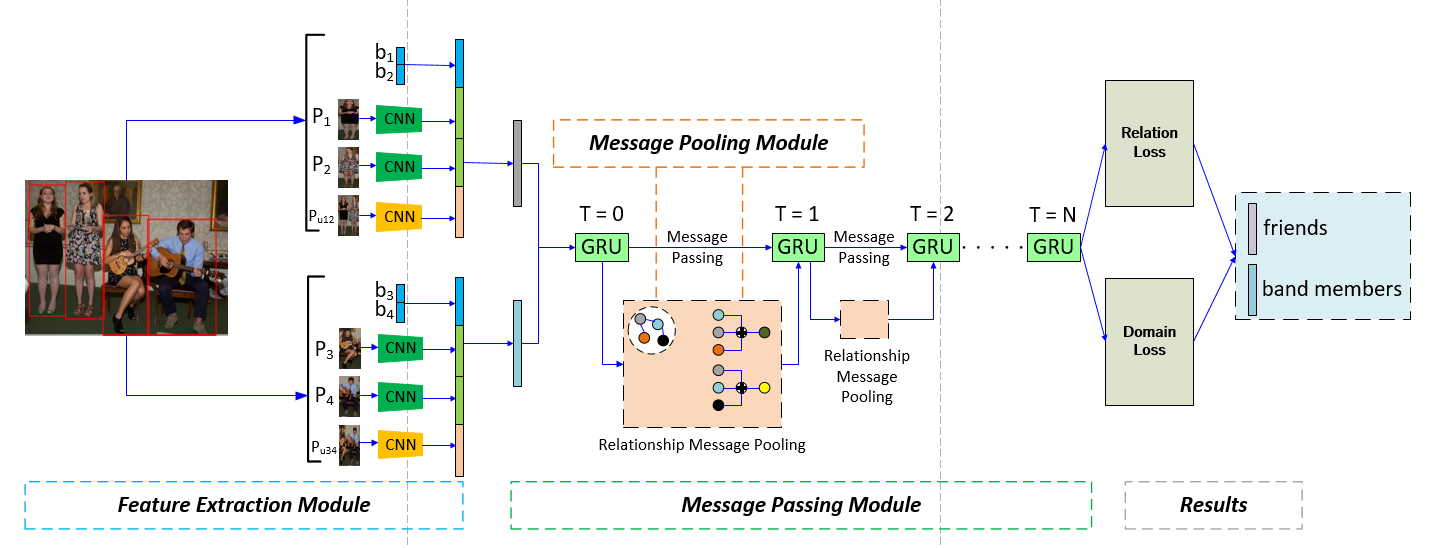
\includegraphics[width=0.98 \textwidth,clip]{model-2.png}
	%\hspace{0.02\textwidth}
	%\vspace*{-0.08cm}
    \caption{PPRN模型的结构示意图}
	\vspace*{-3.5mm}
	\label{fig:model-pprn}
\end{figure}

\section{特征抽取模块}


模型微调是指给定一个预训练模型,这里的预训练网络通常是在大规模标注数据集上训练好的模型,例如常用的预训练模型有Vgg和ResNet。 此时的模型已经能很好的提取大部分图片的信息,比如卷积神经网络的浅层往往是提取基础特征,例如边缘、轮廓等基础特征。深层卷积层提取抽象特征,例如脸型,而最后的全连接层根据特征组合进行连接分类。对于在大规模数据集上已经训练过的模型来说,已经具备了提取浅层特征和深层次抽象特征的能力。基于预训练模型的参数来训练新的数据集能节省很多的计算时间和计算资源,而且还能提升模型的效果。常见的模型微调方法是按照任务的需求设计的分类层替代预训练模型的最后一层,然后以较小的学习率微调前面的所有层,原因是不想过快的扭曲前面已经学习好的特征,然后着重训练最后的分类层。或者冻住预训练模型大多数的网络层,微调少量网络层。

特征提取模块包括物体的特征和人对的特征,对于人对的特征,采用的预训练模型是ResNet-101\cite{he2016deep},本文的做法微调ResNet-101模型的最后2个残差层以及最后的分类层。特征抽取模块的主要目标是提取出输入的图片和人的包围盒坐标区域的图像特征。因此,该模块首先修剪出三个小块,$p_1$ 和$p_2$ 为个体的区域,$p_{u}$ 为两个人区域的并集区域,这些区域的特征包含了用于识别关系的基本组成部分。这些区域首先被调整为大小224 $\times$ 224,然后输入三个ResNet,且提取$p_1$ 和$p_2$ 区域的网络是共享参数的。三个模型最后一个卷积层的输出拼接在一起,形成视觉特征向量$\mathbf{v}_1$。 其次,位置信息是很重要的特征,当模型在识别关系类别中的`` 无关系''时,单纯从视觉特征来判断是很难的,此时位置信息往往能起到很好的区分作用。我们表示一个包围盒$i$ 的特征为$b_i^{pos}$ = $\{ x_{i}^{min}, y_{i}^{min}, x_{i}^{max}, ~y_{i}^{max},~ area_{i} \}$ $\in$ $R^5$。 其中这些值都是相对位置。$x_{i}^{min}$和$y_{i}^{min}$是包围盒的左上角坐标,$x_{i}^{max}$ 和$y_{i}^{max}$是右下角坐标。最后这些特征拼接在一起后通过全连接层形成关系特征向量$\mathbf{v_h}$


\section{利用GRU的推理模块}

\subsection{消息传递模块}
对于一张图片中$n$个人对的关系,通过特征抽取模块,得到了图片中所有人对关系的特征编码,$\{ \mathbf{v_{1}},\mathbf{v_{2}},...,\mathbf{v_{n}} \}$,并且对于一张图片构成的社会关系图谱,是一张全连接图。特征抽取模块得到的关系向量编码通过公式\ref{eq:model-hidden-init}所示,转换到一个低维空间,其中$ \varphi_{rel} $ 可以视为全连接层。
\begin{equation} \label{eq:model-hidden-init}
    \mathbf{x}_{i} = \varphi_{rel} (\mathbf{v_{i}})
\end{equation}

为了学习到图片中的场景信息对关系编码的约束,我们采用了循环神经网络来执行社会关系理解的推理工作。与Zheng\cite{zheng2015conditional}的模型不同的是,我们采用通用的RNN 神经元来计算隐藏层状态。相比较LSTM,GRU少了一个门,因此更加简单并且参数较少,学习起来更快,因此本文采用的是GRU模块。我们采用第t步的隐藏层状态编码表示社会关系图谱中所有关系节点信息,关系节点的向量编码会随着RNN 序列的长度每一步依次更新。而关键的是每一步GRU的输入来自消息池化模块的输出,消息池化模块承担着关系节点间交互的任务。具体细节如公式\ref{eq:model-gru}所示,其中$\mathbf{x}_i$会当作GRU 第一步的输入,并且第一步隐藏层用全0的向量初始化或者随机初始化。这里的$\sigma$和$tanh$分别表示逻辑斯谛回归和双曲正切函数。$\odot$ 操作表示点乘操作,$\bm{r}_t$表示重置门,$\bm{z}_t$表示更新门,下标$t$表示迭代步骤。$\mathbf{W}_r$和$\mathbf{W}_z$ 表示两个门需要的参数,这些参数可训练的。

\begin{equation} \label{eq:model-gru}
\begin{split}
\bm{r}_t &=  \sigma(\bm{W}_{r}[\bm{h}_{t-1}, \bm{x}_t]), \\
\bm{z}_t &=  \sigma(\bm{W}_{z}[\bm{h}_{t-1}, \bm{x}_t]), \\
\hat{\bm{h}_t} &= tanh(\bm{W}[\bm{r}_t \odot \bm{h}_{t-1}, \bm{x}_{t}])\\
\bm{h}_t &= (1 - \bm{z}_t) \odot \bm{h}_{t - 1} + \bm{z}_t \odot \hat{\bm{h}_t} \\
\end{split}
\end{equation}

\subsection{消息池化模块}

消息传递模块利用RNNs解决推理问题,但是在每个迭代步的时候,GRU单元会接受多个来自社会关系图上其他节点的消息,需要有一个聚合模块来将这些信息结合成一个有意义的编码向量。直观来看,常见的池化能实现这个功能,例如常用的最大池化和平均池化。在理解当前图片的社会关系图谱时,但是只利用上下文的结构信息中最相关的那部分是最合理的方式。而本文的消息池化模块也是出于这个目的提出的。下面将会说明简要说明注意力机制的基本情况。如公式\ref{eq:model-mp-atten}所示,其中第$t$ 步的节点$i$的前一步隐藏层状态为$\mathbf{h_{i,t-1}}$,$\mathbf{m}_{i,t}$表示来自其他节点消息的聚合,而$\bm{m}_{i,t}$ 将会作为第$t$ 步中公式
\ref{eq:model-gru}中输入,即$\mathbf{x}_{t}$。其中符号[.]表示两个向量编码的拼接,$\sigma$表示激活函数,$\bm{w}$是需要学习的参数向量,$\bm{h}_{j \to i,t-1}$是节点j在第t-1步时的隐藏层编码,并且等同于
公式\ref{eq:model-gru}中节点j的$\mathbf{h_{t-1}}$

\begin{equation}
    \label{eq:model-mp-atten}
	\bm{m_{i,t}} = ~\sum_{j\neq i} \sigma{(~\bm{w}^T[~\bm{h}_{i,t-1},\bm{h}_{j \to i,t-1}~]) \bm{h}_{j \to i,t-1}}	
\end{equation}

%%%%%%%  注意力机制  %%%%%%%%%%%%

\section{结合周边物体信息模块}

%%%%%%%%%%%%%% 之后写  %%%%%%%%%%% 先空着
本文在模型PPRN,如模型图\ref{fig:model-pprn}的基础上,本文实现了结合周边物体信息模块,模型简称为PPRN+obj,如图\ref{fig:model-atten}。当前模块主要包括两个步骤,利用faster-rcnn 中的RPN网络模块生成物体置信度高的区域,其次利用注意力机制得到关于周边物体区域的特征向量。
\begin{figure}[htpb]
	\centering
	%	\includegraphics[width=0.48 \textwidth, trim=10 10 10 80,clip]{./pic/example_new.pdf}
	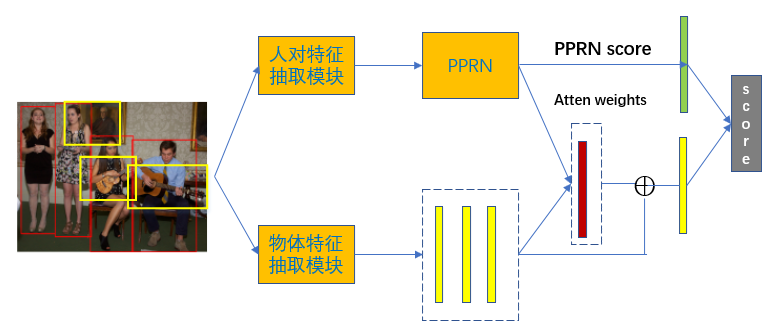
\includegraphics[width=0.98 \textwidth,clip]{model-atten.png}
	%\hspace{0.02\textwidth}
	%\vspace*{-0.08cm}
    \caption{PPRN模型的结构示意图}
	\vspace*{-3.5mm}
	\label{fig:model-atten}
\end{figure}

在一张图片中,往往会存在一些日常见到的物体,例如桌子、电脑、杯子,如果在一张图片中检测到了被杯子、床或者桌子等物体,那么当前的社会关系往往是``家庭''。因此本文在利用关系上下文的基础上,进一步加入周边物体信息来提升效果。但是在PISC 和PIPA-relation数据集中,不包含物体包围盒的标注以及物体类别的标注。COCO\cite{lin2014microsoft}是一个大规模的物体检测的数据集,覆盖了日常常见的80类物体。采用在COCO上预训练好的faster-rcnn 模型,利用其中的区域生成网络。区域生成网络的输入可以是任何大小的图片,输出是一些长方形的检测框,其中每个检测框都带有是否包含物体的得分。由于期望RPN和fast-rcnn 共享vgg\cite{simonyan2015very}的参数(本文采用vgg-16,也可采用其他的预训练模型)生成的特征图,这里的vgg 网络有13个可训练的卷积层。

经典的方法生成检测框都非常耗费时间,例如RCNN和fast-rcnn采用的选择性搜索,而faster-rcnn 抛弃传统的方法,直接从特征图生成检测框,能极大的提升检测的速度。如图\ref{fig:rpn},可以看到RPN网络由两个模块组成,上面的模块为物体的前后景分类,检测的目标为前景。下面的模块为检测框坐标的回归,用于获得更精准的检测框,proposal层结合检测框的坐标和前景类别获取在图上的区域,这两个模块结合起来相当于完成了目标定位的功能。具体执行步骤如下:
\begin{enumerate}
    \item 对于vgg 特征提取模块得到$d$张特征图,因此相当于每个点都是d-dimensions。
    \item 对于$d$张特征图,首先经过$3 \times 3$的卷积核的处理,用于结合周边的空间信息,同时每个点对应的d-dimension不变。
    \item 假设在$d$张特征图中每个点上有k个锚点,每个锚点分为前景和后景,所以在前后景分类中,d-dimension的特征向量转化为一个2k的得分向量,而每个锚点都有四个坐标的偏移量,对于检测框回归模块,特征向量转化为4k的得分向量。其实RPN就是在和原图相同的尺寸上,设置密密麻麻的候选锚点。然后用cnn网络来判断哪些是包含物体目标的前景,那些是不包含物体目标的后景。
    \item 全部锚点框都拿去训练太多了,因此会在锚点框中随机选取128个positive的锚点框和128个negative锚点框用于训练
\end{enumerate}
\begin{figure}[htpb]
	\centering
	%	\includegraphics[width=0.48 \textwidth, trim=10 10 10 80,clip]{./pic/example_new.pdf}
	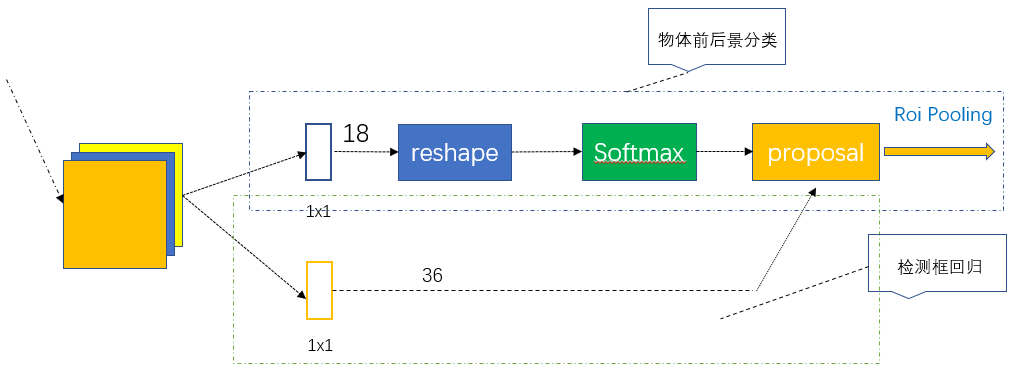
\includegraphics[width=0.95 \textwidth,clip]{rpn.png}
	%\hspace{0.02\textwidth}
	%\vspace*{-0.08cm}
    \caption{RPN网络结构示意图}
	\vspace*{-3.5mm}
	\label{fig:rpn}
\end{figure}
上文提到的锚点框,其示意图如图\ref{fig:anchor},其实就是对于特征图的每个点生成一组检测框,检测框的尺寸由输入的图片的尺寸决定的,在本文中,对于每个检测点生成3种尺寸,每种尺寸3种形状的锚点框。这也是常见的多尺度方法,这9个初始的锚点框的准确度由RPN的区域回归模块处理。对于生成的检测框,因为尺度是原图的尺度大小,需要映射为特征图的尺度大小,Roi pooling层划分出非均匀的网格,对网格采用最大池化然后得到锚点框的特征向量。
\begin{figure}[htpb]
	\centering
	%	\includegraphics[width=0.48 \textwidth, trim=10 10 10 80,clip]{./pic/example_new.pdf}
	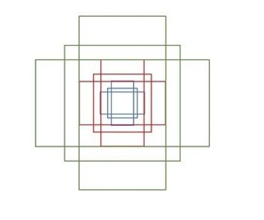
\includegraphics[width=0.50 \textwidth,clip]{anchor.png}
	%\hspace{0.02\textwidth}
	%\vspace*{-0.08cm}
    \caption{anchor示意图}
	\vspace*{-3.5mm}
	\label{fig:anchor}
\end{figure}

利用前文提到的RPN网络,对于图片$\bm{I}$,生成是前景的检测框,得到一组检测框$\bm{P}_{I}$,采用预训练的vgg来得到特征图$conv(I)$,对这里的每个检测框,经过一层Roi pooling 层得到固定长度的物体区域特征$\mathbf{v}$。对于图片所有的检测框,从$conv(I)$生成$\{ \mathbf{v}_{i}|i=1,2,....,N\}$特征向量,对于不同的社会关系关系来说,和它关联的物体是比重是不同的,例如对于关系`` 家庭'',`` 碗''的权重比`` 桌子''的权重大的多,所以我们期望对于不同的物体区域引入不同的权重系数。因此,在当前模块中,引入注意力机制
(attention mechanism),经过消息传递和池化的关系特征编码$\mathbf{v_{top}}$和物体特征编码$\mathbf{v_{i}}$共同决定权重系数的值:
\begin{equation}
    \mu_{i} = \mathbf{u}^{T}~tanh(~\mathbf{W}_{r}v_{top}+\mathbf{W}_{o}v_{i}~)
\end{equation}
\begin{equation}
    \mathbf{a}_{i} = softmax(\mu_i) = \frac{exp(\mu_{i})}{\sum_{j}^{N}exp(\mu_{j})}
\end{equation}
根据关系得到每个物体区域特征的权重后,各个区域权重分别与物体区域的特征编码相乘,如公式\ref{eq:model-obj-wei}所示:
\begin{equation}
    \label{eq:model-obj-wei}
    \mathbf{v_{att}} = \sum_{i}\mu_{i}~\mathbf{v_{i}}
\end{equation}
最终用于分类的的编码由是将消息传递、池化模块得到的关系编码向量$\mathbf{v_{top}}$,和带权物体特征编码特征向量$\mathbf{v_{att}}$,最终的分类层函数如公式\ref{eq:model-cls}:
\begin{equation}
    \label{eq:model-cls}
    \begin{split}
    s^{relation} = \mathbf{W}_{r}[~\mathbf{v}_{top}~,~\mathbf{v}_{att}~] + \mathbf{b}_r \\
    s^{domain} = \mathbf{W}_{d}[~\mathbf{v}_{top}~,~\mathbf{v}_{att}~] + \mathbf{b}_d
    \end{split}
\end{equation}

\section{优化和实现细节}

对于图片\textbf{I}的第k个人对,模型预测出的的得分为$\mathbf{s}_{I,k} \in \mathcal{R}^{|\mathcal{C}|}$,我们采用{\it softmax}函数对得分进行归一化来得到每个类别的概率$\mathbf{p}^{I,k,rel} \in \mathcal{R}^{|\mathcal{C}|}$、
$\mathbf{p}^{I,k,dom} \in \mathcal{R}^{|\mathcal{D}|}$如公式\ref{eq:model-prob-eq}所示:
\begin{equation}
  \label{eq:model-prob-eq}
  \begin{split}
  p_i^{I,k,rel} = \frac{\exp{s_i^{I,k}}}{\sum_{j=1}^{|\mathcal{C}|}{\exp{s_j^{I,k}}}}~, p_i^{I,k,dom} = \frac{\exp{s_i^{I,k}}}{\sum_{j=1}^{|\mathcal{D}|}{\exp{s_j^{I,k}}}} \\
  i=1,2,\dots,|\mathcal{C}|或|\mathcal{D}|
  \end{split}
\end{equation}
这里的$\mathcal{C}$表示社会关系的类别,$|\mathcal{C}|$表示类别的数量,$\mathcal{D}$表示关系域的类别,$|\mathcal{D}|$表示关系域数量。由于是分类任务,模型最终的损失函数如公式\ref{eq:model-loss-eq},其中$N(I)$表示图片I的人对数量,L(.) 表示交叉熵损失函数,$\mathcal{I}$ 表示整个图片集合。
\begin{equation}
  \label{eq:model-loss-eq}
  \mathcal{L} = - \frac{1}{\sum_{I \in \mathcal{I}}\text{N}(I)} \sum_{I \in \mathcal{I}} \sum_{k=1}^{\text{N}(I)} [ \sum_{i=1}^{|\mathcal{C}|} \text{L}(y_{i}^{I,k,rel}, p_{i}^{I,k,rel}) + \sum_{i=1}^{|\mathcal{D}|}\text{L}(y_{i}^{I,k,dom}, p_{i}^{I,k,dom}) ]
\end{equation}

关于本文中提到的预训练模型ResNet-101\footnote{https://download.pytorch.org/models/resnet101-5d3b4d8f.pth}和Vgg-16\footnote{https://download.pytorch.org/models/vgg16-397923af.pth},使用的均是由深度学习框架pytorch\footnote{https://pytorch.org/}提供的。并且在数据集PISC-fine和PIPA-relation中存在类别不均衡问题,PISC-fine类别分布如表
\ref{tab:model-pisc-cls},在实际训练过程中,我们采用常见的过采样和降采样的方法来构造最终的训练集,例如对于PISC-fine中类别为{\it Commercial}的关系,我们扩增3倍的样本,并且这些样本的人对会互换位置(例如p1和p2 是
{\it Commercial},那么新增加的样本为p2和p1也是{\it Commercial})。

在本文中,最开始微调RestNet-101提取人对信息时候采用的是优化方法是SGD,不同数据集在微调所需要的迭代次数是不一样的,同时由于本文模型的输入是以图片为单位,但是不同图片的人对数量是不一样的,所以batch\_size也是不一样的。首先,微调不同数据集所需要迭代次数如表\ref{tab:model-ft-epoch},上文同样提到了,综合考虑到效率和模型效果,本文采用的方法是微调网络最后两个卷积层,其他层的参数冻结,不参与学习更新。其次,利用前面微调的模型参数,固定住,然后只更新消息传递和池化模块的参数,这个步骤采用的优化算法是Adam\cite{kingma2014adam},不断迭代直到模型收敛。在物体的候选区域生成模块,我们设定最多采用30个物体区域。\textbf{PPRN}模型用pytorch实现。对于PISC-coarse和PISC-fine数据集,训练时\footnote{模型运行在一台64位的Linux Ubuntu 16.04LTS系统的机器上,配置是2.20GHz Intel Xeon E5-2630CPU,GeForce GTX1080Ti GPU,以及128G 2133MHz内存}每个mini-batch 会包含24 张图片,每个batch 需要的时间是200ms。对于pipa数据集,mini-batch 的大小设置为16,即每次16 张图片,每个batch 需要的时间大约是300ms。

\begin{table}[htpb]
  \centering
  \caption{PISC-fine类别分布表}
  \label{tab:model-pisc-cls}
  \begin{tabular}{c|c|c|c|c|c|c}
    \toprule
    关系类别 & Friends & Family & Couple & Professional & Commercial & No Relation \\
    \midrule
    样本数量 & 12686 & 788 & 1552 & 20842 & 523 & 11979 \\
    \bottomrule
  \end{tabular}
\end{table}


\begin{table}[htpb]
  \centering
  \caption{fine-tune ResNet-101需要的迭代轮数}
  \label{tab:model-ft-epoch}
  \begin{tabular}{c|c|c|c}
    \toprule
    数据集 & PISC-coarse & PISC-fine  & PIPA-relation \\
    \midrule
    预训练迭代轮数 & 17 & 24 & 2 \\
    \midrule
    \bottomrule
  \end{tabular}
\end{table}

\section{本章小结}

本章提出了一个全新的基于消息传递机制的关系网络,简称\textbf{PPRN}。\textbf{PPRN}模型是一个端到端的架构,主要由四个部分构成,特征抽取模块、消息传递模块、消息池化模块、结合物体信息模块,模块之间是串联的,并且它们的作用和分工不同。

特征抽取模块的作用是输入一张图片,图片中所有人身体的检测框坐标,提取出其中表示人对关系的基本特征编码,包括单个人区域、两个人的联合区域和位置信息,特点是利用两个不同的预训练模型来处理单人区域和两个人的联合区域,我们同时结合了图像特征和位置特征,特征提取采用的是微调后的ResNet-101。基于特征提取模块得到的向量编码已经能够表达人对间的社会关系了,而消息传递和池化模块的作用是结合当前图片的场景信息进行关系类别推理,学习到图片中不同人对关系之间约束。学习这个约束的原因是,在一张图片中,场景往往是固定的,所以图片中不同人对的社会关系之间是相互影响的。本文采用以GRU为基础的RNN 作为推理模型,每次迭代时,利用注意力机制结合图片中其它人对关系的编码,实现不同人对关系间的消息传递,RNN最后一步的隐藏层编码表示所有的人对关系。

然后,本章在Dual-glance模型的基础上,实现了类似的结合物体信息模块。物体信息指的是利用基于大规模训练集的预训练faster-rcnn模型,RPN网络生成图片的物体检测框,包含物体的概率大于一定的阀值。本章详细的介绍了RPN网络的细节,如何生这些检测框坐标。最后提取出这部分上下文物体区域的信息。因为不同物体区域对和不同的社会关系的相关度不一样,同样利用注意力机制为每个物体区域的特征编码分配权重。

最后,本章介绍了优化和实现细节。模型包括两部分的损失,关系损失和关系域损失,损失函数采用常见的交叉熵损失函数,并且针对PISC-fine和PIPA-relation数据集的数据不均衡问题,进行数据上的过采样和降采样。模型的训练过程是分段式的,包括微调预训练模型和本文提出的模块训练两部分,结合不同的学习率和优化方法模型得以训练。





\clearpage{\pagestyle{empty}\cleardoublepage}
%\include{body/mns}
%\clearpage{\pagestyle{empty}\cleardoublepage}       %本有
% !Mode:: "TeX:UTF-8"

\chapter{实验设计与分析}
\label{ch:exp}

本章将利用常见的社会关系理解的数据集对上一章提到的PPRN模型进行检测任务的验证,具体来说即对图片中两个标定的坐标人的关系类别。本章首先介绍当前所用到的两个数据集训练/验证/测试的数据分布情况,数据集的特点。再介绍若干对比模型,介绍实验的参数设置,然后分别对实验结果进行说明和分析,并且对其中消息池化进行了不同实现方法的对比。最后通过案例研究的方法来分析PPRN模型在关系补全任务中发挥的效果。

\section{数据集}

\subsection{数据集简介}

现有的大规模社会关系理解的数据集主要有两个:分别是PIPA-relation\cite{sun2017a}数据集和PISC\cite{li2017dual-glance}数据集,下面简单介绍这两个数据集。

PISC数据集全称是People in social Context,它是Sun等人在2017年通过人工标注平台得到的数据集,这些图片主要来自Visual Genome\cite{krishna2017visual}、COCO\cite{lin2014microsoft}、YFCC100M\cite{thomee2016yfcc100m}、instagram 和twitter等社交网站,Google和Bing商业搜索引擎。从这数据额的来源可以保证数据集的图片是足够高的方差的,人的面部表情,以及场景类型。PISC数据集包含22670张图片以及对应的社会关系标注,在PISC数据集上,又包含两个粒度的识别任务,coarse-level和fine-level。如图\ref{fig:exp-pisc-r}所示的划分方式,先是粗粒度的,再到细粒度的关系类别。
\begin{figure}[htpb]
	\centering
	%	\includegraphics[width=0.48 \textwidth, trim=10 10 10 80,clip]{./pic/example_new.pdf}
	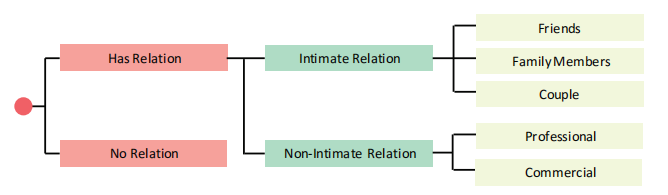
\includegraphics[width=0.98 \textwidth,clip]{pisc-split.png}
	%\hspace{0.02\textwidth}
	%\vspace*{-0.08cm}
    \caption{PISC的关系划分}
	\vspace*{-3.5mm}
	\label{fig:exp-pisc-r}
\end{figure}

PIPA-relation数据集的全称是People in Photo Album Relation,总共包括37107张图片。同样是人工标注的数据集,基于社会关系理论\cite{bugental2000acquisition}划分的,Sun\cite{sun2017a}详细的给出了每个关系域的特征。然后所有的社会关系划分为5个关系域,在构建数据集的过程中,这5个关系域划分为16种社会关系,五个关系域分别是Attachment domain、Reciprocity domain、Mating domain、Hierarchical power domain和Coalitional groups domain。Attach domain划分为father-child,mother-child,Grandpa-grandchild和grandma-grandchild,Reciprocity domain划分为friends, siblings和classmates。Mating domain只包含单条关系lovers/spouses。Hierarchical power domain划分为presenter-audience, teacher-student, trainer-trainee and leader-subordinate。Coalitional groups domain划分为band members, dance team members, sport team members and colleagues。

数据集的情况如表\ref{tab:exp-pisc-statistic},``Train''表示训练集图片的数量,``Valid''和``Test''分别表示验证和测试集的图片数量。``\#train''表示训练集人对的数量,``\#valid''和``\#test''分别表示验证和测试集的人对数量。
\begin{table}[htpb]
  \centering
  \caption{PISC、PIPA-relation数据集的统计列表}
  \setlength{\tabcolsep}{4.5mm}
  \label{tab:exp-pisc-statistic}
  \begin{tabular}{c|c|c|c|c|c|c}
    \toprule
    数据集 & Train & Valid & Test & \#train  &  \#valid &  \#test  \\
    \midrule
    PISC-coarse & 13142 & 4000 & 4000 & 14536 & 25636 & 15497   \\
    \midrule
    PISC-fine &  16828 & 500 & 1250 & 55400 & 1505 & 3691 \\
    \midrule
    PIPA-relation & 5857 & 261 & 2452 & 13729 & 709 & 5106 \\
    \bottomrule
  \end{tabular}
\end{table}

\subsection{数据集分析}

对于数据集PISC-coarse、PISC-fine和PIPA-relation,本文做了基本的数据集分析,如表\ref{tab:exp-data-analysis-1},其中``Sui''表示一张图片有多个人对的比例,``Unsui''则表示一张图片只有一个人对的百分比。·``Single Rel''一张图片包含的关系类别只有一种,``Multi Rel''表示一张图片包含多种关系。从表统计数据可以得到两个结论,从``Sui''和``Unsui''来看,绝大多数的图片是包含多个人对的,从``Multi Rel''来看,一张图片的关系种类往往是相同的,因为直观来看,给定场景下的社会关系时稳定的。例如,假如张图片是一个会议的场景,那么其中往往会有多个人对,并且这些人对间的社会关系往往是``
colleagues''或``presenter audience''。
\begin{table}[htpb]
  \centering
  \caption{PISC 和 PIPA-relation统计分析}
  \label{tab:exp-data-analysis-1}
  \begin{tabular}{c|c|p{0.9cm}<{\centering}|p{0.9cm}<{\centering}||p{0.9cm}<{\centering}|p{0.9cm}<{\centering}}
    \midrule
    \multicolumn{2}{c|}{Dataset} & Sui. & Unsui. & \tabincell{c}{Single\\Rel.} & \tabincell{c}{Multi\\Rel.} \\
    \midrule
    \multirow{2}*{PISC} & coarse & 87.1 & 12.9 & 79.9 & 20.1\\
    \cline{2-6}
    ~ & fine & 83.9 & 16.1 & 86.4 & 13.6 \\
    \midrule
    \multicolumn{2}{c|}{PIPA-relation 16} & 71.9 & 28.1 & 94.9 & 5.1 \\
    \midrule
  \end{tabular}
\end{table}

此外,对于关系类别这项统计,本文做了进一步工作,并且发现一张图片的关系种类大多只是一种,少部分是两种。如图\ref{fig:exp-statistic}所示,在PISC-coarse中,大约79.9\%的图片是只有一种关系类别,20.0\%的图片有含有两个关系。

\begin{figure}[htpb]
	\centering
	%	\includegraphics[width=0.48 \textwidth, trim=10 10 10 80,clip]{./pic/example_new.pdf}
	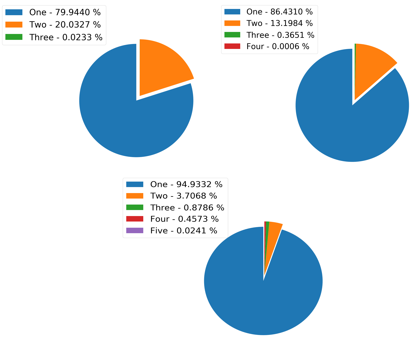
\includegraphics[width=0.65 \textwidth,clip]{ppp.png}
	%\hspace{0.02\textwidth}
	%\vspace*{-0.08cm}
    \caption{数据集的关系类别统计}
	\vspace*{-3.5mm}
	\label{fig:exp-statistic}
\end{figure}

\section{实验设置}

在预训练模型,包括ResNet-101和Vgg-16最后一层的维度都是是4096,经过全连接层,在消息传递和池化模块的中的编码长度为512。池化模块中注意力机制的attention_size=30,结合周边物体信息模块中注意力机制的attention_size=30


\section{实验对比}



%\clearpage{\pagestyle{empty}\cleardoublepage}       %本有
%\include{body/experiment}
%\clearpage{\pagestyle{empty}\cleardoublepage}       %本有
%% !Mode:: "TeX:UTF-8"

\chapter{总结与展望}
\label{ch:conclusion}

\section{本文总结}

近年来,随着深度学习方法在计算机视觉领域的广泛应用,基于图像理解的应用也逐渐增多,随之各种任务数据集的构造和应用的落地。但是基于图片的高层次推理和理解仍然是待解决的难题,例如图像的视觉理解,以及本文关注的社会关系理解人物。与此同时,随着人们的研究的深入进展,如何利用更少的信息和人工干预来提升社会关系理解任务的效果是一大挑战。此外,在视觉理解领域的另外一个方向,基于消息传递、图网络等技术生成的场景图谱在各大领域的成功应用,例如图像问答和图像检索。但是由于两者存在许多不同点,在社会关系理解领域引入场景图谱生成的方法是另外一大挑战。
本文的主要工作和贡献点总结如下:
\begin{enumerate}
    \item 针对提出的挑战,本文首先弄明白了现有关系理解方法的研究现状,分析了现有方法的研究现状,现有方法忽略了一张图片人对的关系之间互相影响的信息。即现有的方法需要额外的检测标注。其次,调研了现有场景图谱生成工作,明确了社会关系理解和场景图谱理解的各项概念。社会关系理解的目的是识别出给定一对人的的社会关系。
    \item 接下来,本文充分考虑了同一场景下多个人对的社会关系间互相这一因素,提出了人对关系网络(PPRN),这是首个在社会关系理解任务上引入人对关系的交互模型。针对性的设计了迭代的消息传递和池化模块来融合交互信息。主要包括3个模块:视觉特征提取模块、消息传递和消息池化模块。视觉特征提取模块主要是由2部分组成,个体CNN和联合CNN,采用的是预训练的ResNet-101,结合位置信息后得到关于人对关系的特征编码向量。传递和消息池化主要是利用迭代的门控循环神经网络实现推理,并且在每个神经元之前都采用消息池化的机制融合其他人对的信息。此外,本文还实现了融合周边物体信息模块,得到物体特征的特征编码向量,进一步验证模型的效果。
    \item 为了验证本文所提出的PPRN模型的有效性,本文在两个大规模的数据集上进行了相关的实验、主要的评价指标包括每个关系类别热召回率以及mAP。采用每个关系类别的召回率是因为每个关系类别的训练样本存在数据不均衡的情况,与此同时还需要在训练集进行过采样和降采样。mAP综合考虑召回率和准确率的效果。实验结果说明PPRN模型在社会关系理解任务上展现了优秀的性能,说明了考虑人对关系上下文的重要性。同时,基于低层次特征抽取模型得到的编码,再进行高层次的推理,是本文的核心点。
\end{enumerate}

\section{研究展望}

基于对社会关系理解的分析以及本文提出对各项相关任务的分析、相关技术的考量,基于本文的基础,未来的研究可以是以下方面开展:
\begin{enumerate}
    \item 将现有的视觉关系检测的工作引入到社会关系检测中,人们对场景图谱的研究相当深入,视觉三元组在图像问答和图片检索上发挥了很大的作用。同时,现有的社会关系理解的``人''并没有id或者名称,可以结合人脸识别的方法进一步给识别出人的id,建立一个整体的图像社会关系图谱。
    \item 现有模型挖掘的特征包括周边的物体上下文、关系上下为难均为场景这一粒度的,可以尝试加入更细粒度的。例如人的性别特征,这样的特征在区分{\it Friends}和{\it Couple}等容易混淆的气密关系的时候时能起到关键的作用,例如相同性别一般不可能是{\it Couple},而是其他的亲密关系。
    \item 可以将视觉领域的社会关系理解拓展到视频领域的,
\end{enumerate}


%\clearpage{\pagestyle{empty}\cleardoublepage}       %本有

%%%%%%%%%%  参考文献  %%%%%%%%%%
\titleformat{\chapter}{\centering\sihao\hei}{\chaptername}{2em}{}
\defaultfont
%\bibliographystyle{TJUThesis}
\bibliographystyle{references/TJUThesis}        % bst文件名,注意不要后缀
\phantomsection
\markboth{参考文献}{参考文献}
\addcontentsline{toc}{chapter}{参考文献}        % 参考文献加入到中文目录
%\nocite{*}                                     % 若将此命令屏蔽掉,则未引用的文献不会出现在文后的参考文献中
\bibliography{references/reference}             % bib文件名
\include{references/reference}
\clearpage{\pagestyle{empty}\cleardoublepage}   %本有
\include{appendix/cmpresult-A}               %附录 实验结果表
\clearpage{\pagestyle{empty}\cleardoublepage}
\include{appendix/cmpresult-B}               %附录 实验结果表
\clearpage{\pagestyle{empty}\cleardoublepage}
%% !Mode:: "TeX:UTF-8"

\markboth{攻读硕士学位期间发表学术论文情况}{攻读硕士学位期间发表学术论文情况}
\addcontentsline{toc}{chapter}{攻读硕士学位期间发表学术论文情况}
%\setcounter{page}{1}       % 如果需要从该页开始从 1 开始编页,则取消该注释
\chapter*{攻读硕士学位期间发表学术论文情况}

\begin{enumerate}
	% 盲审时
	\item Understanding Social Relationship with Person-pair Relations. 投稿于IJCAI-2019(ccf推荐A类会议),学生第一作者,审稿中
    \item 一种基于二次主题空间投影的场景图谱低维空间嵌入方法; (学生第一作者,申请未公开)
	% 提交时
	%\item Authors. The paper title [J/C...]. Publish whereabout, 2014, 21(3): 288-291. (提交时)
\end{enumerate}

% 仍然有页码
%\thispagestyle{empty}
                       % 攻读硕士学位期间发表学术论文情况
\clearpage{\pagestyle{empty}\cleardoublepage}   %本有
% !Mode:: "TeX:UTF-8"

\markboth{致\quad 谢}{致\quad 谢}
\addcontentsline{toc}{chapter}{致\quad 谢} % 添加到目录中
\chapter*{致\quad 谢}

谨此向我的导师张三教授致以衷心的感谢和崇高的敬意!本论文的工作是在张老师的悉心指导下完成的。在传授予我专业知识和宝贵经验的同时,张老师以其严谨的治学态度和精益求精的工作作风不断促进论文相关工作的进行,使我受益匪浅。
 
在攻读硕士的这三年里,导师和实验室的同学们不仅为我创造了优越的科研和学习环境,使我得以在计算机科学领域中自由翱翔,同时在思想上、人生态度和意志品质方面给予了谆谆教诲,这些教益必将激励着我在今后的人生道路上奋勇向前。特别感谢实验室的甲师兄、乙同学以及其他师弟师妹,他们不仅在学术上给了我许多指引和建议,而且在生活上予以帮助,从他们身上我学到了很多知识。

感谢王五老师及其实验室的同学在领域一、领域二方面的学习给予我的帮助。他们开创性的研究拓展了我的学术视野,无数次的争论和探讨使我的研究工作有了长足的进展。

由衷感谢我的室友A、B和C同学,以及其他经常到我们宿舍进行学习交流的D、E、F和G同学,是他们令我的学习生活都更加充满动力。
衷心的感谢我的父母和其他亲朋好友对我的关心、支持和理解,没有他们对我的关心、鼓励和支持,我无法完成现在的硕士学业。 

最后,感谢所有曾经教育和帮助过我的所有老师。衷心地感谢为评阅本论文而付出宝贵时间和辛勤劳动的专家和教授们!

% 如果需要加名字和日期(日期根据生成文档日期变更)
\begin{flushright}
  \begin{tabular}{cl}
    李四 & \\
    二零一四年\CJKnumber{\the\month}月\CJKnumber{\the\day}日 & 
  \end{tabular}
\end{flushright}

             % 致谢
%\clearpage{\pagestyle{empty}\cleardoublepage}
\clearpage
\end{CJK*}                                      % 结束中文字体使用
\end{document}                                  % 结束全文
